% Created 2026-07-10 Fri 01:28
% Intended LaTeX compiler: xelatex
\documentclass[14pt]{article}
\usepackage{graphicx}
\usepackage{longtable}
\usepackage{wrapfig}
\usepackage{rotating}
\usepackage[normalem]{ulem}
\usepackage{capt-of}
\usepackage{hyperref}
\usepackage{graphicx}
\usepackage{hyperref}
\usepackage{listings}
\usepackage[margin=0.7in]{geometry}
\usepackage{booktabs}
\usepackage{fontspec}
\setmainfont{Hack}
\setmonofont{Hack}
\setcounter{secnumdepth}{4}
\date{}
\title{NextLearn — Project Documentation}
\hypersetup{
 pdfauthor={},
 pdftitle={NextLearn — Project Documentation},
 pdfkeywords={},
 pdfsubject={},
 pdfcreator={Emacs 30.2 (Org mode 9.7.11)}, 
 pdflang={English}}
\begin{document}

\maketitle
\setcounter{tocdepth}{2}
\tableofcontents

\newpage
\section{Cover Page}
\label{sec:org11180c0}
\begin{center}

\includegraphics[width=300]{./screenshots/nextlearn-logo-high-res.png}
\end{center}

\begin{center}
{\Huge \textbf{NextLearn}} \\[1em]
{\Large Distraction-Free Digital Study Environment} \\[2em]
{\large Project Documentation} \\[3em]

\textbf{Zagazig University} \\
Faculty of Computer Science and Informatics \\[1em]
IT department \\[1em]

\textbf{Author:} Hassan Ahmad Darwish (NSB) \\[1em]

\textbf{Version:} 1.0.0
\end{center}

\newpage
\section{Introduction}
\label{sec:org0473083}
\subsection{Problem Statement}
\label{sec:org7c6d16f}
Modern learners face a fragmented landscape of study tools. The typical
student juggles multiple applications --- a note-taking app for course
content, a flashcard app for memorization, a quiz platform for
self-assessment, and a calendar or timer for study sessions. Each tool
has its own data format, its own synchronization mechanism, and
critically --- its own set of distractions.

The core problem is twofold:

\begin{enumerate}
\item \textbf{\textbf{Context Switching Cost}} — Moving between tools breaks the mental
state of deep study. Every application boundary is an opportunity
for distraction: notifications, advertisements, social features, and
unrelated content compete for the learner's attention.

\item \textbf{\textbf{Vendor Lock-in and Data Portability}} — Most learning platforms
store content in proprietary databases. Exporting to a different
tool is difficult or impossible. The learner's intellectual work is
trapped inside a single ecosystem.

\item \textbf{\textbf{Customization Constraints}} — Mainstream study apps offer limited
keyboard customization, few theming options, and no scripting
capabilities. Users who prefer keyboard-centric workflows (Vim,
Emacs) or require accessibility accommodations are underserved.

\item \textbf{\textbf{AI Integration Fragmentation}} — When AI-powered features exist,
they are typically tied to subscription tiers, have opaque
algorithms, and cannot be used with locally-stored content.
\end{enumerate}

\newpage
\subsection{Solution \& Significance of Work}
\label{sec:org0dc68de}
NextLearn addresses these problems by providing a single, distraction-free
desktop application that integrates:

\begin{itemize}
\item \textbf{\textbf{File-based content management}} — Decks are plain-text \texttt{.md}, \texttt{.org},
or \texttt{.txt} files stored in a local vault. No proprietary database for
content. Your study material is portable, version-controllable (git),
and editable in any text editor.

\item \textbf{\textbf{Keyboard-centric navigation}} — Three built-in keybinding profiles
(Vim, Emacs, VS Code) with multi-key chords, a command palette, and
a customizable keybinding system. Every action is accessible without
touching the mouse.

\item \textbf{\textbf{Offline-first architecture}} — All core features (deck reading,
search, study, heatmap tracking, focus timer) work without an
internet connection. Only optional AI features (tag inference,
flashcard generation, MCQ generation) require the network.

\item \textbf{\textbf{Integrated AI with local-first workflow}} — Google Gemini API is
used for optional AI assistance: tag suggestion, flashcard creation,
and MCQ quiz generation. The AI writes to local files that the user
can review, edit, and control.

\item \textbf{\textbf{Built-in assessment tools}} — MCQ quizzes with interactive WebView
rendering, Anki-compatible flashcard export, and a Pomodoro focus
timer — all within the same application window.
\end{itemize}


The significance of this work lies in demonstrating that a single-d
developer can build a professional-grade, cross-platform study
environment using free and open-source technologies (.NET, Avalonia UI,
SQLite), integrate AI services without compromising local control, and
create a keyboard-first user experience that rivals mainstream
applications.

\newpage
\subsection{Existing Solutions — Limitations vs NextLearn Advantages}
\label{sec:orgd04ac6b}
\subsubsection{anki}
\label{sec:org7452925}
\begin{center}
\begin{tabular}{ll}
Aspect & Anki\\
\hline
Content Format & Proprietary .apkg\\
Keyboard Navigation & Basic shortcuts\\
AI Integration & No native AI\\
Assessment & SRS flashcards only\\
Offline Capability & Full\\
Customizability & Add-ons only\\
Cross-Platform & Windows/macOS/Linux/Android\\
Study Streak Tracking & Basic\\
File Portability & Requires export\\
Cost & Free\\
Focus / Timer & No\\
\end{tabular}
\end{center}
\subsubsection{obsidian.md}
\label{sec:org934970c}
\begin{center}
\begin{tabular}{ll}
Aspect & Obsidian\\
\hline
Content Format & Markdown files\\
Keyboard Navigation & Limited\\
AI Integration & Community plugins only\\
Assessment & No native quizzes\\
Offline Capability & Full\\
Customizability & Plugin system\\
Cross-Platform & Windows/macOS/Linux/mobile\\
Study Streak Tracking & Community plugin\\
File Portability & Native (plain markdown)\\
Cost & Free (sync paid)\\
Focus / Timer & Community plugin\\
\end{tabular}
\end{center}

\newpage
\subsubsection{superMemo}
\label{sec:orgb933226}
\begin{center}
\begin{tabular}{lll}
Aspect & Roam Research & SuperMemo\\
\hline
Content Format & Proprietary & Proprietary .sm\\
Keyboard Navigation & Moderate & Minimal\\
AI Integration & Limited AI & No\\
Assessment & No & SRS + some tests\\
Offline Capability & Limited & Full\\
Customizability & Limited & Minimal\\
Cross-Platform & Web-based & Windows (limited)\\
Study Streak Tracking & No & Basic\\
File Portability & Export only & Export only\\
Cost & Subscription & Paid\\
Focus / Timer & No & No\\
\end{tabular}
\end{center}
\subsubsection{nextlearn}
\label{sec:orgb7d70d1}
\begin{center}
\begin{tabular}{ll}
Aspect & NextLearn\\
\hline
Content Format & .md / .org / .txt files\\
Keyboard Navigation & Vim/Emacs/VS Code profiles\\
AI Integration & Built-in Gemini (tags, MCQs)\\
Assessment & Flashcards + MCQ + Focus Timer\\
Offline Capability & Full (AI optional)\\
Customizability & YAML config + keybinding YAML\\
Cross-Platform & Linux/macOS (Windows planned)\\
Study Streak Tracking & Built-in heatmap + daily log\\
File Portability & Native (plain text)\\
Cost & Free (open source)\\
Focus / Timer & Built-in Pomodoro + todos\\
\end{tabular}
\end{center}



\begin{itemize}
\item Key advantages of NextLearn over existing solutions:
\begin{enumerate}
\item Single-application integration of reading, flashcards, quizzes, timer, and streak tracking — eliminating context switching.
\item Plain-text file format as the source of truth — not a database dump.
\item Keyboard profiles that match the user's existing muscle memory.
\item Deterministic deck identity via SHA256 file path hashing — progress survives file renames and OS reinstallation.
\item AI features that write to the user's local file system, not a locked cloud service.
\end{enumerate}
\end{itemize}

\newpage
\subsection{Background}
\label{sec:org7b0bf8e}
\subsubsection{Linux Philosophy and Customizability}
\label{sec:org975e53e}
NextLearn was developed on primarily on ArchLinux. The design
philosophy draws heavily from the Unix tradition:

\begin{itemize}
\item \textbf{\textbf{Do one thing well}} — The app is a study tool, not a notes app,
not a project manager, not a social network.
\item \textbf{\textbf{Plain text as universal interface}} — Deck files are plain text.
Users can edit them with any tool, version them with git, and
transform them with shell scripts.
\item \textbf{\textbf{Composability}} — The app is designed to fit into a Linux workflow.
File manager integration, CLI-paired deck creation, and
git-backed version history are first-class concerns.
\item \textbf{\textbf{Transparency}} — All data lives in standard locations:

(\texttt{\textasciitilde{}/.config/nextlearn/}, \texttt{\textasciitilde{}/nextlearn/decks/}). No hidden databases
or opaque binary formats.
\end{itemize}
\subsubsection{Vim and Emacs Influence}
\label{sec:org1590477}
The keyboard shortcut system is directly inspired by the two great
traditions of modal editing:

\begin{itemize}
\item \textbf{\textbf{Vim profile}} — Single-key navigation (j/k for scroll, n/p for
pages), modal context awareness, and the \texttt{g} leader key for chords.
The command palette (activated by \texttt{:}) mirrors Vim's command-line
mode.

\item \textbf{\textbf{Emacs profile}} — Chords with modifier keys (\texttt{C-n}, \texttt{C-p}), prefix
key sequences (\texttt{C-x}, \texttt{C-c}), and the \texttt{M-x} command palette. The
chord display indicator shows pending key sequences with a 500ms
timeout, reminiscent of Emacs's \texttt{C-g} cancel mechanism.

\item \textbf{\textbf{VS Code profile}} — Familiar shortcuts for users coming from the
most popular modern editor (\texttt{Ctrl+Shift+P} for command palette,
\texttt{Ctrl+B} for sidebar, \texttt{Ctrl+W} for close).
\end{itemize}

Supporting these three profiles means users can be productive within
seconds of first launch — no need to learn a new keybinding system from
scratch.

\newpage
\subsubsection{.NET Ecosystem and Avalonia UI}
\label{sec:org5e52830}
The technical foundation is .NET 10.0 with Avalonia UI, chosen for:

\begin{itemize}
\item Cross-platform desktop rendering (Linux, macOS, Windows) from a single
codebase.
\item XAML-based declarative UI with MVVM architecture via
CommunityToolkit.Mvvm (source-generated observable properties and
relay commands).
\item Direct hardware acceleration via Skia rendering backend.
\item NativeWebView control for HTML content rendering, enabling rich
text display with KaTeX math and highlight.js syntax highlighting.
\end{itemize}
\subsection{Methodology}
\label{sec:orgcfe238d}
\subsubsection{Chosen Methodology — Kanban (Lean/Agile)}
\label{sec:org3181a49}
NextLearn was developed using a Kanban-style approach, documented in
\texttt{plan-todos.org} (1351 lines of feature planning). The choice was driven
by:

\begin{itemize}
\item Single-developer project — no need for sprint ceremonies or
team coordination.
\item Evolving scope — features were added based on user (self) feedback and
practical need, not a fixed requirements document.
\item Continuous delivery — every feature went through the same pipeline:
plan → implement → test → document → commit.
\end{itemize}

The Kanban board is informal but effective:
\begin{verbatim}
TODO (plan-todos.org) → In Progress (active work) → Done (committed)
\end{verbatim}

Each feature entry in \texttt{plan-todos.org} includes:
\begin{itemize}
\item Detailed specification with rationale
\item File-by-file change list
\item Edge case table
\item Test impact assessment
\item Progress UI step table (where applicable)
\end{itemize}

\newpage
\subsubsection{Other Methodologies Considered}
\label{sec:org01a2ab8}
\begin{center}
\begin{tabular}{lll}
Methodology & Considered & Rejected Because\\
\hline
Waterfall & Yes & Scope evolved during development\\
Scrum & Yes & Overhead for single developer\\
Spiral & Yes & Risk analysis overhead not justified\\
RAD & Yes & Prototyping not needed — domain understood\\
Extreme (XP) & Yes & Pair programming not applicable\\
\end{tabular}
\end{center}
\subsection{Project Objectives}
\label{sec:org1ebb6eb}
\begin{enumerate}
\item \textbf{\textbf{Study Environment}} — Provide a distraction-free, keyboard-centric
application for reading markdown and org-mode decks as paginated
slides.

\item \textbf{\textbf{File-First Architecture}} — Use plain text files as the source of
truth for all study content. No proprietary content format.

\item \textbf{\textbf{Cross-Platform Desktop}} — Target Linux (primary), macOS, and
Windows using a single .NET/Avalonia codebase.

\item \textbf{\textbf{Integrated Learning Tools}} — Include flashcard generation, MCQ
quizzes, and a Pomodoro timer within the same application.

\item \textbf{\textbf{Optional AI Assistance}} — Integrate AI services (Google Gemini)
for tag suggestion, flashcard creation, and quiz generation without
requiring internet connectivity for core features.

\item \textbf{\textbf{Progress Tracking}} — Track study streaks, daily minutes, and
page-level progress with a persistent heatmap visualization.

\item \textbf{\textbf{Customizability}} — Provide configurable keybinding profiles,
dark/light theme switching, and font/text-size adjustment without
requiring plugin installation.

\item \textbf{\textbf{Keyboard-First Design}} — Support three major keybinding profiles
(Vim, Emacs, VS Code) with multi-key chords and a command palette
for full mouse-free operation.
\end{enumerate}

\newpage
\section{Planning \& Requirements}
\label{sec:org5591668}
\subsection{Project State \& Scope}
\label{sec:org5295131}
NextLearn is currently in active development with the following scope
constraints:

\begin{itemize}
\item \textbf{\textbf{Platform Focus}}: Linux (primary). WebView rendering uses
\texttt{libwpewebkit-2.0} and related WPE dependencies available on Linux.
macOS builds pass CI but are less tested. Windows is not currently
supported (requires WebView2; the author lacks a Windows machine for
consistent testing).

\item \textbf{\textbf{Single-User Mode}}: The app creates a local "Guest" user on first
launch. No multi-user or cloud sync features.

\item \textbf{\textbf{Optional AI}}: All Google Gemini API features (tag inference,
flashcard generation, MCQ generation) are optional. The app functions
fully without them.

\item \textbf{\textbf{Offline-First}}: Core features require zero network connectivity.
Only AI features depend on internet access.
\end{itemize}
\subsection{Development Tools \& Environment}
\label{sec:org6167900}
The project was developed using a deliberately minimal toolchain.
Experience with the tools shaped both the development process and the
design philosophy:

\begin{center}
\begin{tabular}{ll}
Tool & Purpose\\
\hline
VS Code & Primary IDE for C\# and XAML development\\
Vim & Fast edits, configuration file changes, shell\\
Emacs (org-mode) & Documentation and planning\\
Git (CLI) & Version control\\
JetBrains Rider & Tried as alternative IDE\\
Avalonia Hot Reload & XAML live preview\\
\end{tabular}
\end{center}





\begin{center}
\begin{tabular}{ll}
Tool & Notes\\
\hline
VS Code & With C\# Dev Kit, Avalonia, and Markdown plugins\\
Vim & Used for quick file modifications\\
Emacs (org-mode) & All .org files (README, changelog, bugs, plan-todos) created in Emacs\\
Git (CLI) & Command-line git, no GUI wrapper\\
JetBrains Rider & Abandoned: too heavy for the low-end development machine\\
Avalonia Hot Reload & Discovered late in development cycle; never used in practice\\
\end{tabular}
\end{center}

\begin{quote}
The "Avalonia Hot Reload" discovery is notable: the author was unaware
that Avalonia supported XAML live reloading until approximately 80\% of
the core UI was complete. By that point, the edit-compile-run cycle was
already embedded in the workflow, and adopting hot reload mid-project
offered marginal benefit. This is documented as a lesson for future
projects.
\end{quote}

\newpage
\subsection{Technology Stack}
\label{sec:orgea59909}
\subsubsection{versions}
\label{sec:org2d689f2}
\begin{center}
\begin{tabular}{ll}
Technology & Version\\
\hline
.NET & 10.0\\
Avalonia UI & 11.3.12\\
CommunityToolkit.Mvvm & 8.2.1\\
Entity Framework Core & 8.0.0\\
SQLite & (EF Core)\\
Serilog & 4.3.1\\
NativeWebView & 0.1.0-alpha.3\\
NativeWebView.Platform.Linux & 0.1.0-alpha.3\\
YamlDotNet & 18.0.0\\
highlight.js & 11.11.1\\
KaTeX & (bundled)\\
StyleCop.Analyzers & 1.2.0-beta.556\\
Google Gemini API & REST\\
xUnit & (latest)\\
FluentAssertions & (latest)\\
NSubstitute & (latest)\\
\end{tabular}
\end{center}
\subsubsection{why used}
\label{sec:orgadf4ee0}
\begin{center}
\begin{tabular}{ll}
Technology & Purpose\\
\hline
.NET & Runtime framework\\
Avalonia UI & Cross-platform desktop UI framework\\
CommunityToolkit.Mvvm & Source-generated MVVM pattern\\
Entity Framework Core & ORM for SQLite\\
SQLite & Embedded local database\\
Serilog & Structured logging (file + console)\\
NativeWebView & System WebView HTML rendering\\
NativeWebView.Platform.Linux & Linux WebView backend (WPE WebKit)\\
YamlDotNet & YAML serialization (settings, keybindings, focus timer data)\\
highlight.js & syntax highlighting (52 langs, bundled as custom-highlight.js)\\
KaTeX & \LaTeX{} math rendering (katex.min.js, katex.min.css, auto-render)\\
StyleCop.Analyzers & C\# code style enforcement\\
Google Gemini API & AI tag inference, flashcard generation, MCQ generation\\
xUnit & Unit testing framework\\
FluentAssertions & Readable test assertions\\
NSubstitute & Mocking framework\\
\end{tabular}
\end{center}
\subsection{System Dependencies (Linux runtime)}
\label{sec:org43cc321}
\begin{itemize}
\item libwpewebkit-2.0 (WebView engine)
\item libwpe-1.0
\item libWPEBackend-fdo-1.0
\item Wayland auto-detection: \texttt{XDG\_SESSION\_TYPE=wayland} → X11 fallback
via \texttt{UseSkia().UseX11()}
\end{itemize}

\newpage
\subsection{Functional Requirements}
\label{sec:org9a746f6}
\subsubsection{Core Deck Management}
\label{sec:org8a299d3}
\begin{itemize}
\item FR-01: Read \texttt{.md}, \texttt{.org}, and \texttt{.txt} files from a configurable vault
directory (default \texttt{\textasciitilde{}/nextlearn/decks/})
\item FR-02: Parse YAML frontmatter for title, description, and tags in
\texttt{.md} and \texttt{.org} files
\item FR-03: Split decks into paginated slides based on heading hierarchy
(\texttt{\#} / \texttt{\#\#} for sections and pages)
\item FR-04: Auto-refresh deck list when files change via FileSystemWatcher
\item FR-05: Search decks by title, description, filename, and tags (with
prefix operators \texttt{file:}, \texttt{title:}, \texttt{desc:}, \texttt{tags:})
\item FR-06: Regex toggle for search
\item FR-07: Pin/archive/unpin/unarchive decks via file rename convention
(\texttt{+.md} for pinned, \texttt{.md\textasciitilde{}} for archived)
\item FR-08: Deterministic deck identity via SHA256 file path hash
\item FR-09: Recursive vault scanning with subdirectory support
\item FR-10: Open decks folder in system file manager
\end{itemize}
\subsubsection{Study \& Navigation}
\label{sec:orgf22f6b8}
:PROPERTIES:
:NEXT:
\begin{itemize}
\item FR-11: Page-by-page learning with previous/next navigation
\item FR-12: Section breadcrumb showing current position in deck hierarchy
\item FR-13: Rendered markdown and org-mode content in WebView
\item FR-14: Code syntax highlighting via highlight.js (52 languages)
\item FR-15: Markdown/Org table rendering
\item FR-16: Image rendering (inline + floating image overlay with zoom,
navigation, invert colors)
\item FR-17: Clickable http/https links and wiki-style deck links
\item FR-18: Quote block rendering (= > = syntax)
\item FR-19: Org general block rendering (\texttt{\#+BEGIN\_*} / \texttt{\#+END\_*})
\item FR-20: Falcon Eye table of contents (auto-generated TOC page per deck)
\item FR-21: Todo checkbox rendering ([ ], [x], [-], [\textasciitilde{}])
\item FR-22: Copy button on code and quote blocks
\item FR-23: \LaTeX{} math rendering via KaTeX (inline \texttt{\$..\$}, display
\texttt{\$\$..\$\$})
\item FR-24: Go-to-page dialog (Ctrl+G)
\item FR-25: Text zoom in/out/reset (Ctrl+Shift++/-/0)
\end{itemize}

\newpage
\subsubsection{Keyboard System}
\label{sec:orga0e9a4a}
\begin{itemize}
\item FR-26: Three built-in keybinding profiles (Vim, Emacs, VS Code)
\item FR-27: Customizable keybinding via YAML config file
\item FR-28: Multi-key chord support with 500ms timeout and visual
indicator
\item FR-29: Command palette with fuzzy search (activated by \texttt{:} or \texttt{M-x})
\item FR-30: Shortcuts handbook (auto-generated from current profile)
\item FR-31: 67 keyboard action types across multiple contexts (Learning,
Home, ImageOverlay, McqQuiz)
\item FR-32: Esc-based overlay closing priority chain
\end{itemize}
\subsubsection{AI Features (Google Gemini)}
\label{sec:org73be0da}
\begin{itemize}
\item FR-33: AI tag inference — suggest 2--15 tags per deck, diff preview,
apply to frontmatter (supports 7 tag formats)
\item FR-34: Anki flashcard generation — Basic (TSV) and Cloze (\{\{c1::\}\})
modes, separate prompts, save to \texttt{.basic.txt} / \texttt{.cloze.txt} files
\item FR-35: MCQ quiz generation — AI-generated questions, interactive
quiz in dedicated WebView (2x2 option grid, timer, scoring)
\item FR-36: Model auto-discovery and fallback chain (gemini-2.5-flash →
gemini-2.0-flash → etc.)
\item FR-37: Exponential retry with backoff (1s, 5s, 10s, 20s, 40s, 80s)
\item FR-38: Token estimation with 700K truncation limit
\end{itemize}
\subsubsection{Progress \& Analytics}
\label{sec:orge69c230}
\begin{itemize}
\item FR-39: Per-user progress tracking (current page, completed decks)
\item FR-40: Daily activity tracking (pages viewed, minutes learned)
\item FR-41: Study streak heatmap (snake layout, 6-level orange, green for
today)
\item FR-42: Stable progress across restarts (SQLite persistence)
\end{itemize}

\newpage
\subsubsection{Focus Timer}
\label{sec:orgd9cde49}
\begin{itemize}
\item FR-43: Pomodoro-style work/break countdown timer
\item FR-44: Configurable work/break durations in settings
\item FR-45: Persistent todo list (CRUD) with YAML persistence
\item FR-46: Session history log
\item FR-47: Sound notification at session end
\end{itemize}
\subsubsection{Settings \& Configuration}
\label{sec:orgeddd3ad}
\begin{itemize}
\item FR-48: Theme switching (Dark/Light) with live preview
\item FR-49: Configurable decks, MCQs, and flashcards paths
\item FR-50: Gemini API key configuration with status indicator
\item FR-51: Configurable font selection
\item FR-52: Settings persistence in \texttt{settings.yaml}
\item FR-53: Save/Reset settings
\end{itemize}
\subsection{Non-Functional Requirements}
\label{sec:orgebafb31}
\begin{center}
\begin{tabular}{ll}
Requirement & Description\\
\hline
Offline Operation & Core features must work without internet\\
Startup Time & App must launch within 3 seconds\\
File Change Responsiveness & Deck list must refresh within 500ms of file change\\
Memory Footprint & Must run on 4GB RAM systems (low-end machine target)\\
Single-User Architecture & No multi-user sync or authentication required\\
Data Durability & No data loss on crash — SQLite WAL mode, YAML atomic writes\\
Keyboard-Only Operation & All features accessible without mouse\\
Open Data Format & All user data in plain text (.md, .org, .yaml, .txt)\\
Cross-Platform Compatible & Builds on Linux (x64), macOS (arm64), Windows (x64)\\
No Vendor Lock-In & User can stop using the app and keep all data intact\\
CI/CD Integration & Automated build + test on every push via GitHub Actions\\
Single-File Distribution & Published as self-contained executable\\
\end{tabular}
\end{center}

\newpage
\section{System Design}
\label{sec:org6407cc4}
\subsection{System Architecture}
\label{sec:orgdae105a}
NextLearn follows a layered MVVM (Model-View-ViewModel) architecture
with a single-window UI pattern.

\begin{center}
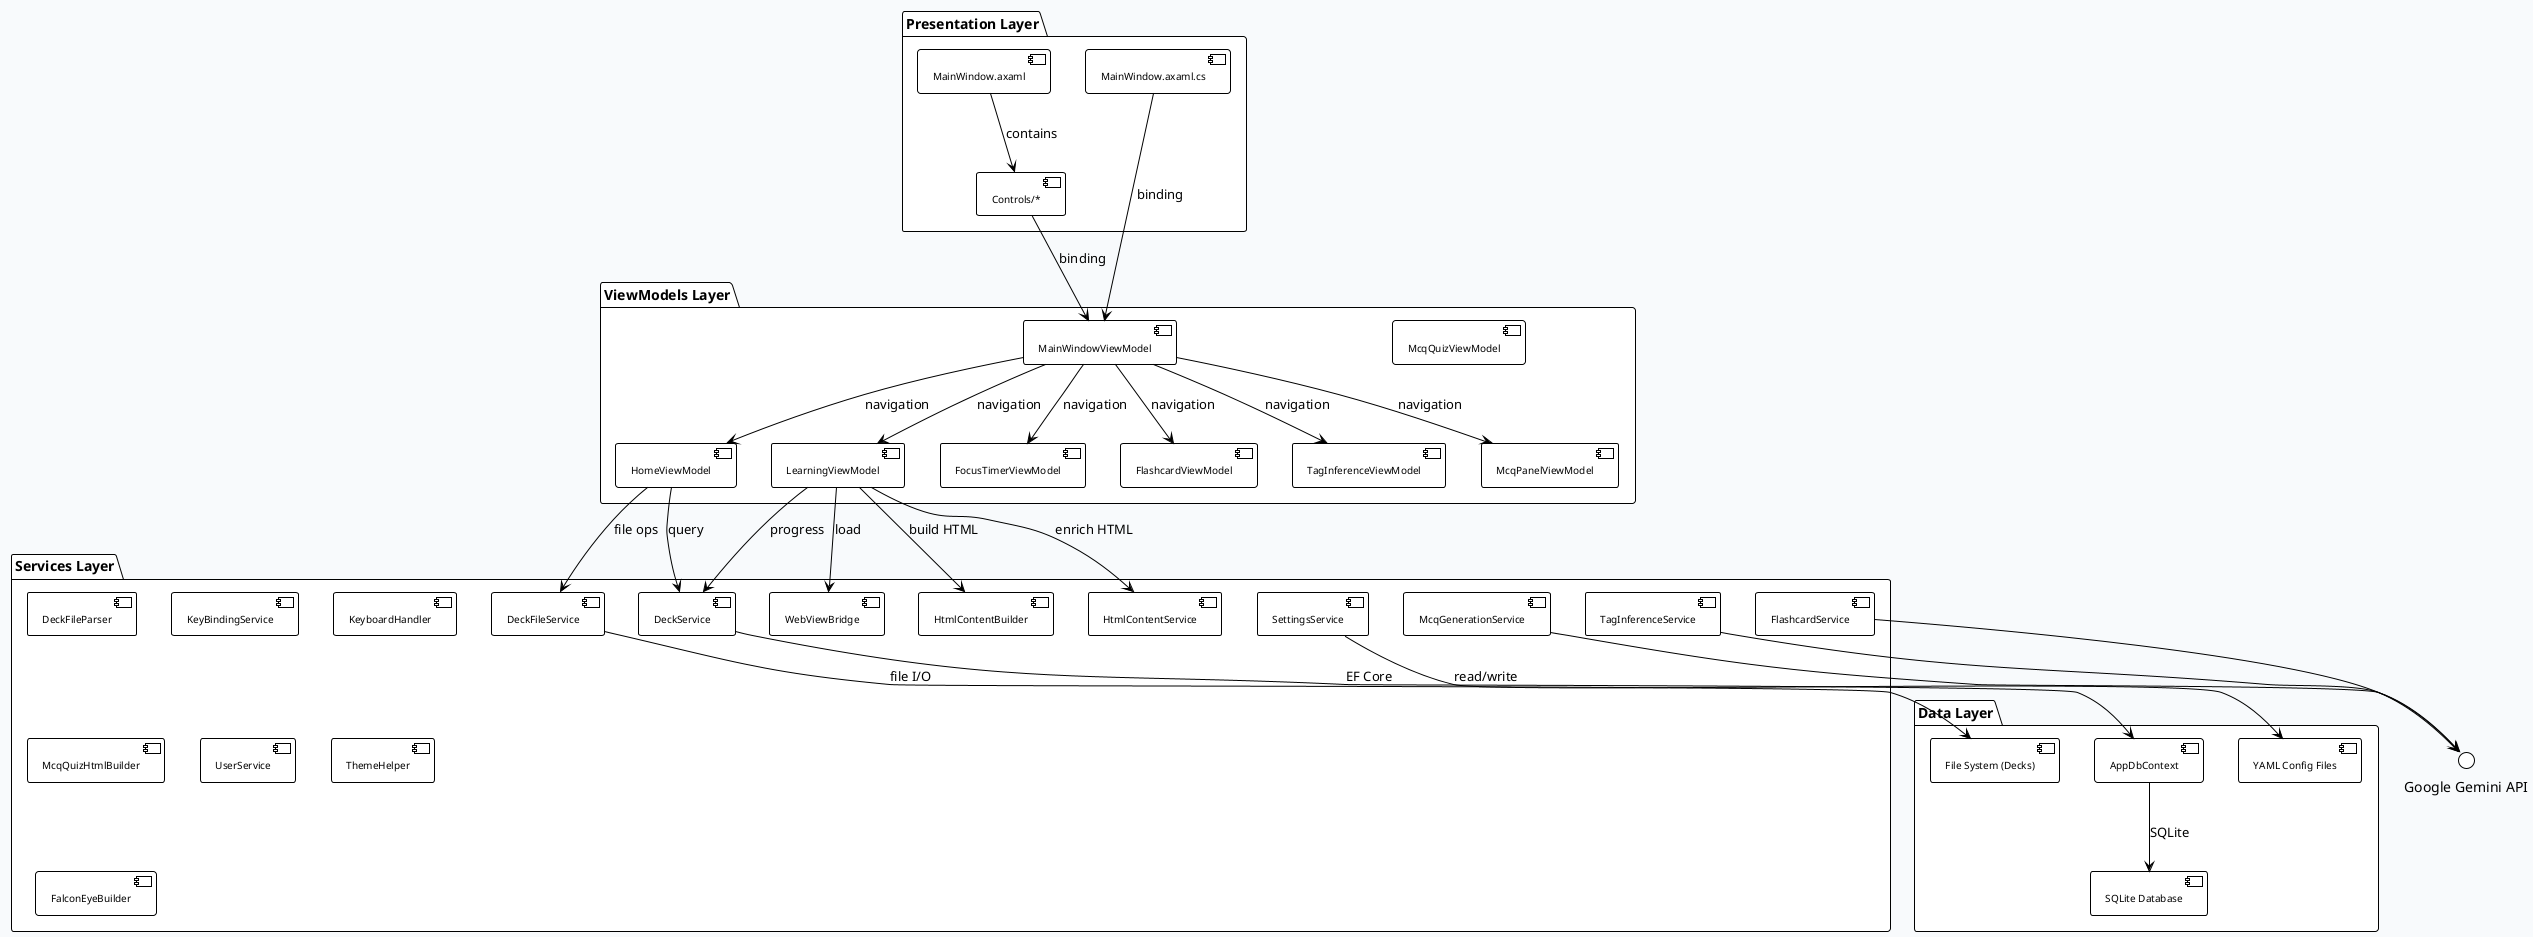
\includegraphics[width=550]{diagrams/architecture.png}
\end{center}
\subsubsection{Single-Window UI Pattern}
\label{sec:org955bcee}
Unlike most desktop applications that use multiple windows or a
navigation framework, NextLearn uses a single \texttt{MainWindow.axaml} with
approximately 15 boolean visibility flags to show/hide panels:

\begin{verbatim}
IsLearning        → learning view (WebView content + pagination)
IsSettingsOpen    → settings overlay
IsSidebarOpen     → sidebar panel
IsTagInferenceOpen → tag inference panel
IsFlashcardOpen   → flashcard generation panel
IsMcqOpen         → MCQ quiz panel (3 tabs)
IsTimerOpen       → focus timer panel
IsPinnedViewOpen   → pinned decks overlay
IsArchivedViewOpen → archived decks overlay
IsHeatmapOpen     → streak heatmap overlay
IsCommandPaletteOpen → command palette
IsShortcutsHandbookOpen → shortcuts handbook
IsGoToPageOpen    → go-to-page dialog
IsImageOverlayOpen → image overlay
IsDeckLinkPromptOpen → deck link navigation prompt
\end{verbatim}

This approach eliminates navigation stacks and keeps the memory
footprint minimal. Only one panel is visible at a time (except sidebar,
which overlays).

\newpage
\subsection{UML Diagrams}
\label{sec:orged0fa8a}
\subsubsection{Use Case Diagram (make it vertical \#baka) \#ok}
\label{sec:orga8b7354}
\begin{center}
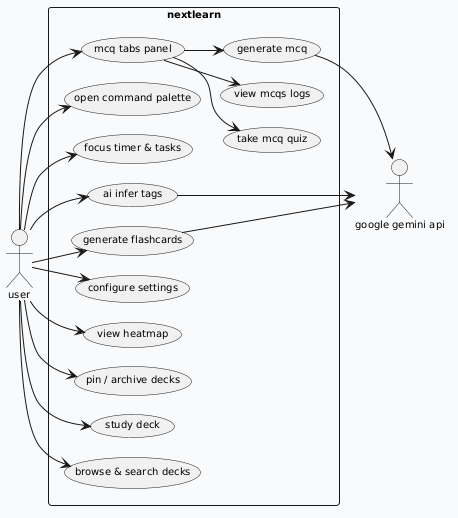
\includegraphics[width=550]{diagrams/usecase.png}
\end{center}

\newpage
\subsubsection{Class Diagram — Core Models}
\label{sec:org33d57e1}
\begin{center}
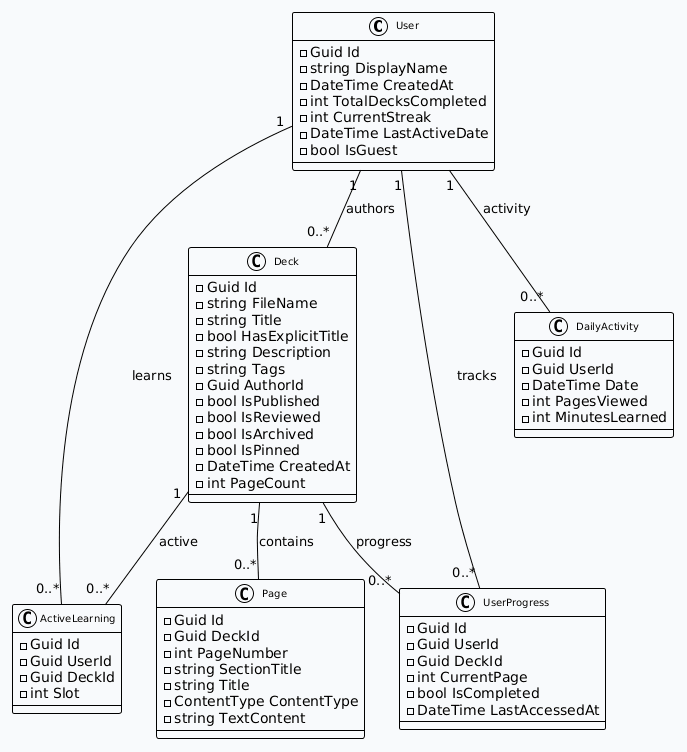
\includegraphics[width=.9\linewidth]{diagrams/class-models.png}
\end{center}
\subsubsection{Class Diagram — Core Services (need this one to vertical \#baka)}
\label{sec:org808fd49}
\newpage
\begin{center}
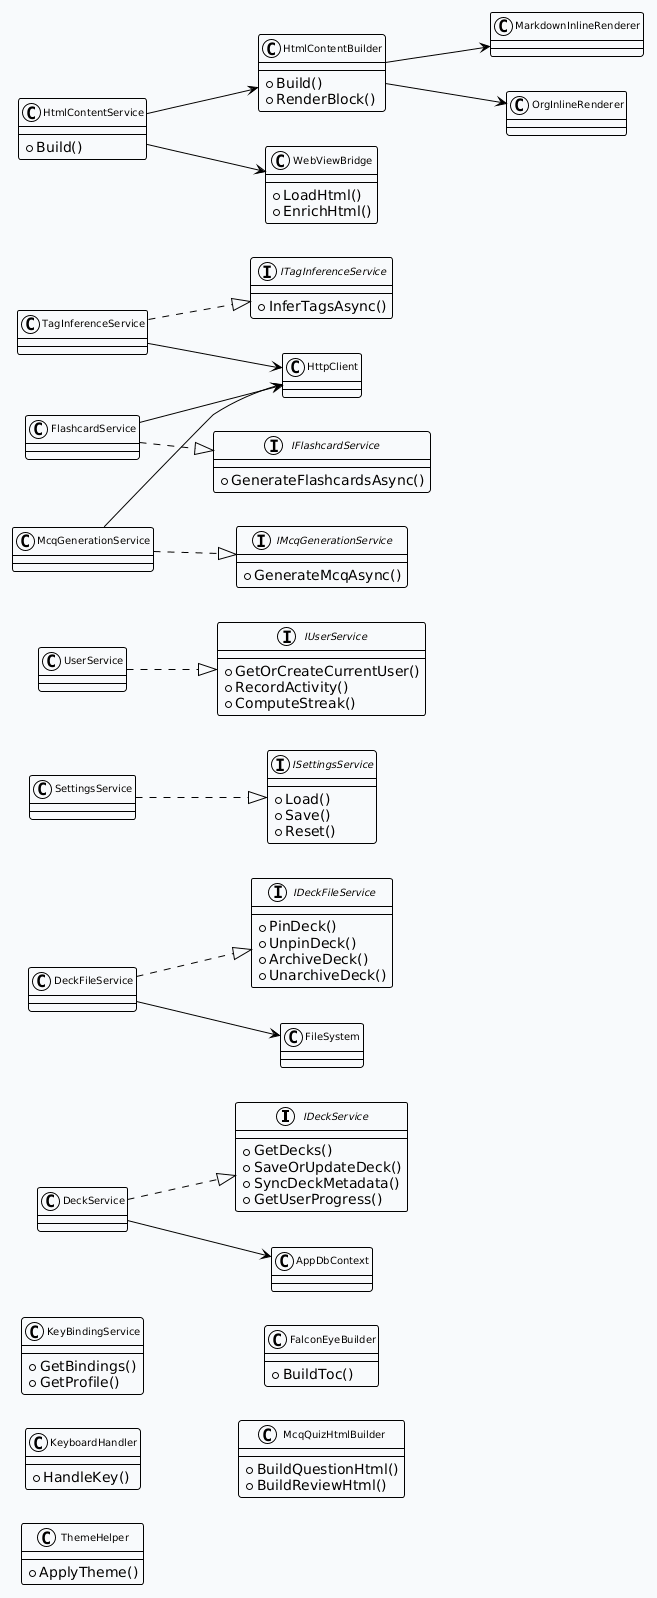
\includegraphics[height=700]{diagrams/class-services.png}
\end{center}
\subsubsection{Activity Diagram — Study Flow}
\label{sec:org57bff1f}
\begin{center}
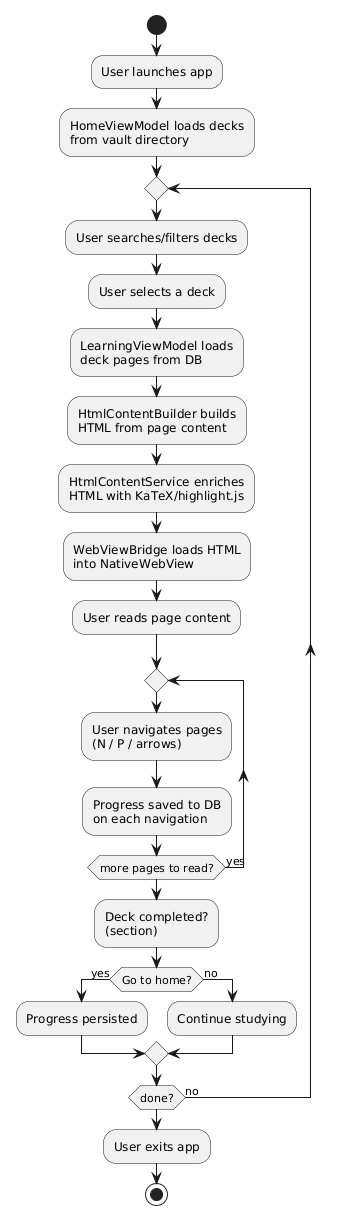
\includegraphics[height=700]{diagrams/activity-study.png}
\end{center}
\subsubsection{Activity Diagram — MCQ Quiz Flow}
\label{sec:org22cfb88}
\begin{center}
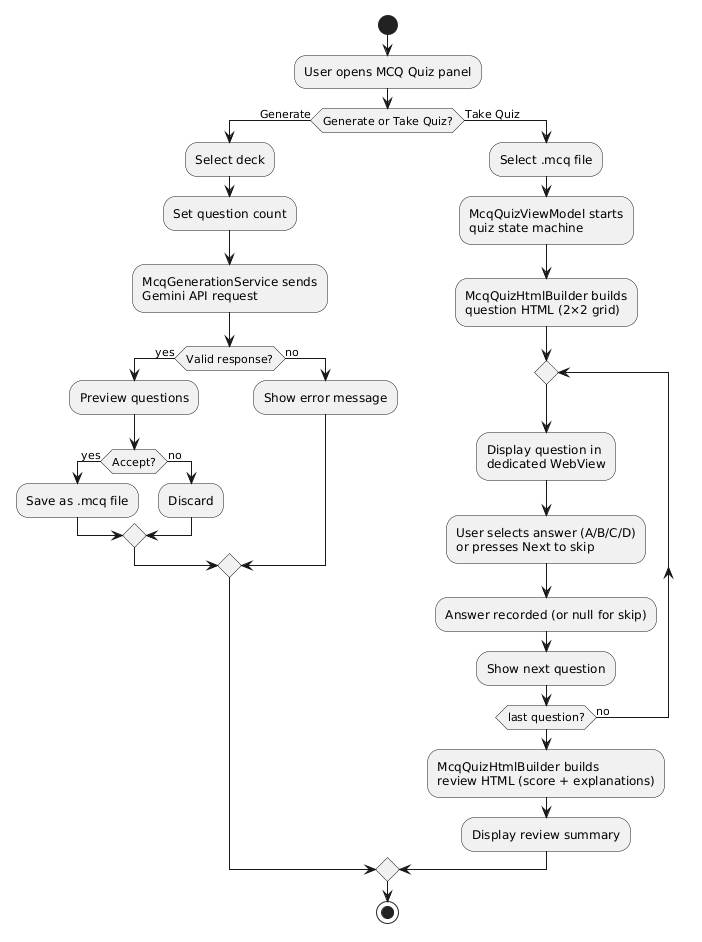
\includegraphics[width=.9\linewidth]{diagrams/activity-mcq.png}
\end{center}
\subsubsection{Sequence Diagram — AI Tag Inference}
\label{sec:orga9ea655}
\begin{center}
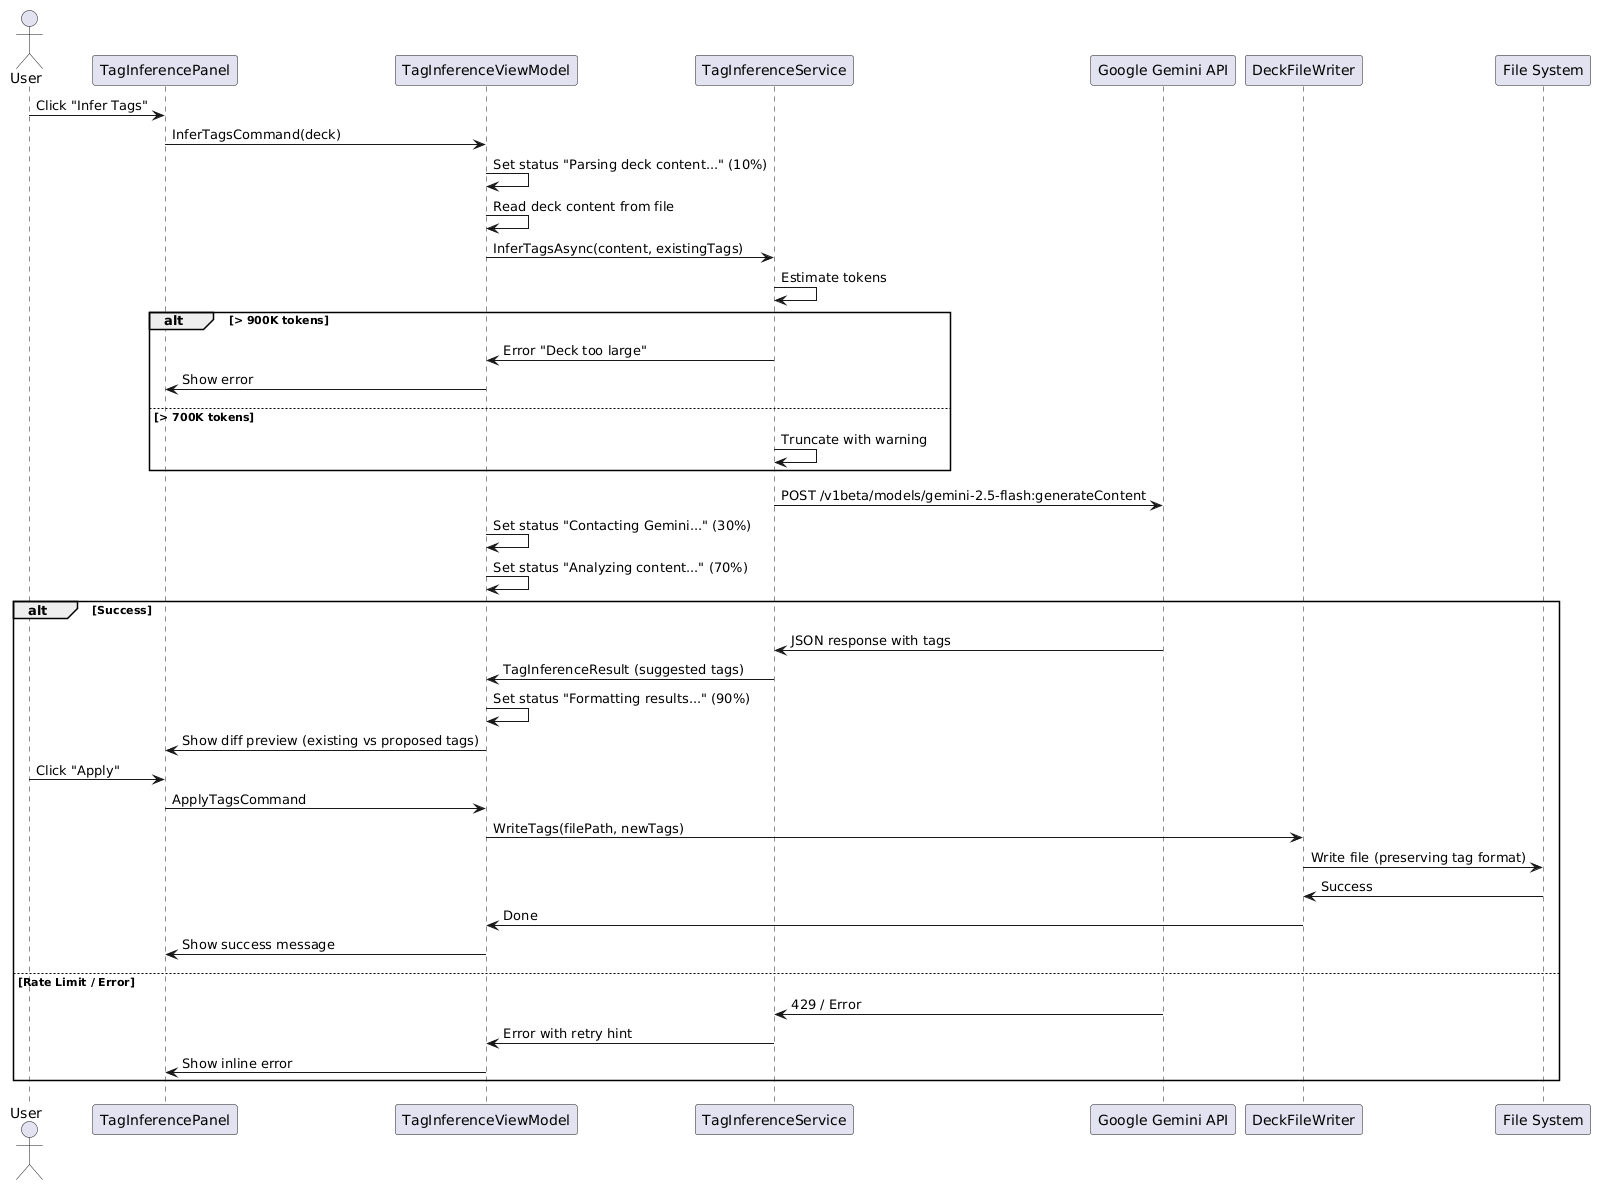
\includegraphics[width=550]{diagrams/sequence-tag-inference.png}
\end{center}
\subsubsection{ER Diagram — Database Schema}
\label{sec:org2f0b43f}
\begin{center}
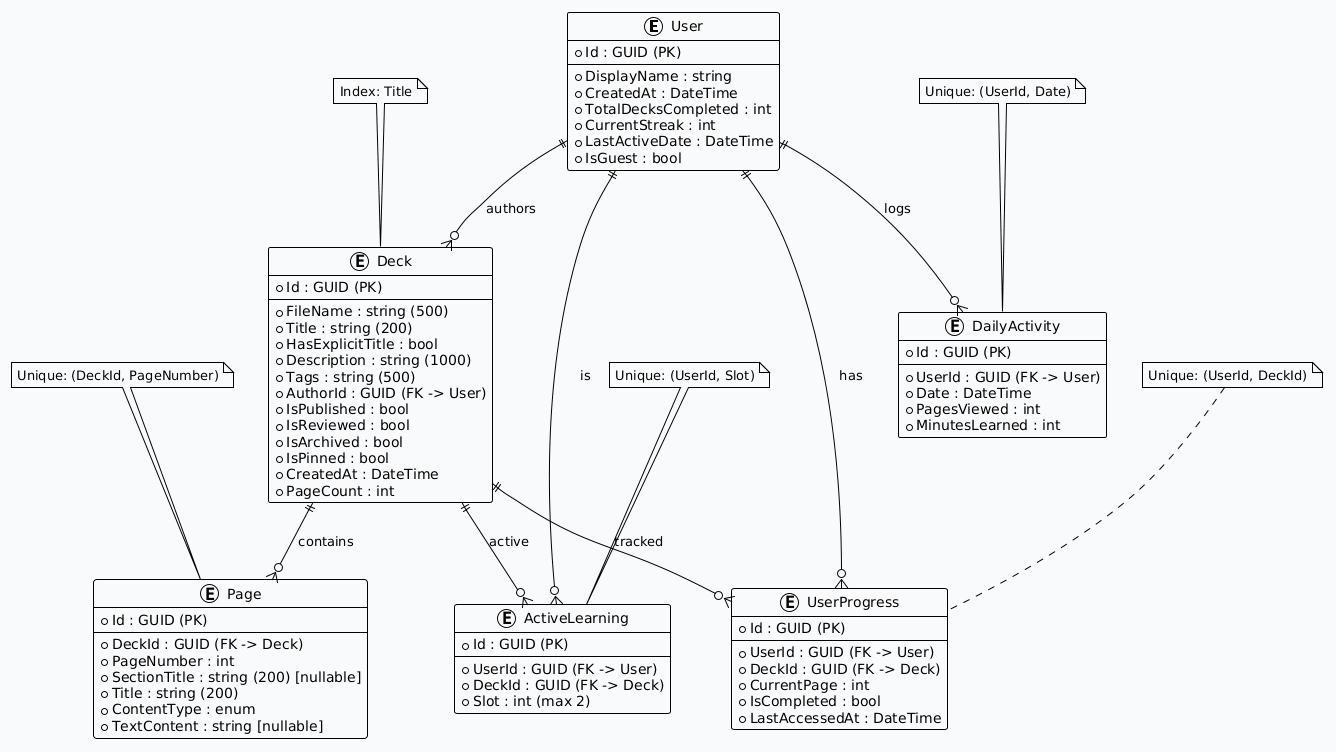
\includegraphics[width=.9\linewidth]{diagrams/er-database.png}
\end{center}
\subsection{Database Design}
\label{sec:orgec4a1ef}
The SQLite database is stored at \texttt{\textasciitilde{}/.config/nextlearn/nextlearn.db} and
contains six tables managed by Entity Framework Core 8.0.0. The database
stores only metadata and progress — deck content lives in the file system.
\subsubsection{Table: Users}
\label{sec:orgb2432f3}
\begin{verbatim}
Column              Type     Constraints Notes
──────────────────────────────────────────────────────
Id                  GUID     PK          Auto-generated
DisplayName         string   NOT NULL    Default "Guest"
CreatedAt           DateTime NOT NULL
TotalDecksCompleted int      NOT NULL    Counter
CurrentStreak       int      NOT NULL    Computed from daily activity
LastActiveDate      DateTime NOT NULL
IsGuest             bool     NOT NULL    Always true (single-user)
\end{verbatim}

\newpage
\subsubsection{Table: Decks}
\label{sec:org20b2e17}
\begin{verbatim}
Column           Type        Constraints         Notes
──────────────────────────────────────────────────────────────
Id               GUID        PK                  Deterministic (SHA256 of path)
FileName         string(500) NOT NULL            Relative vault path
Title            string(200) NOT NULL            Indexed
HasExplicitTitle bool        NOT NULL
Description      string(1000) NOT NULL
Tags             string(500) NOT NULL            Comma-separated
AuthorId         GUID        FK → Users.Id
IsPublished      bool        NOT NULL
IsReviewed       bool        NOT NULL
IsArchived       bool        NOT NULL            '~' suffix convention
IsPinned         bool        NOT NULL            '+' prefix convention
CreatedAt        DateTime    NOT NULL
PageCount        int         NOT NULL
\end{verbatim}
\subsubsection{Table: Pages}
\label{sec:org915d3aa}
\begin{verbatim}
Column              Type        Constraints     Notes
───────────────────────────────────────────────────────────
Id                  GUID        PK
DeckId              GUID        FK → Decks.Id
PageNumber          int         NOT NULL        1-based
SectionTitle        string(200) NULLABLE        From # heading
Title               string(200) NOT NULL        From ## or first line
ContentType         enum        NOT NULL        Text (only value)
TextContent         string?     NULLABLE        Raw markdown/org

UNIQUE INDEX: (DeckId, PageNumber)
\end{verbatim}
\subsubsection{Table: UserProgress}
\label{sec:org2c39474}
\begin{verbatim}
Column              Type        Constraints    Notes
──────────────────────────────────────────────────────────
Id                  GUID        PK
UserId              GUID        FK → Users.Id
DeckId              GUID        FK → Decks.Id
CurrentPage         int         NOT NULL       Default 1
IsCompleted         bool        NOT NULL          
LastAccessedAt      DateTime    NOT NULL          

UNIQUE INDEX: (UserId, DeckId)
\end{verbatim}

\newpage
\subsubsection{Table: ActiveLearning}
\label{sec:orgf9a84d5}
\begin{verbatim}
Column              Type        Constraints     Notes
───────────────────────────────────────────────────────────
Id                  GUID        PK
UserId              GUID        FK → Users.Id
DeckId              GUID        FK → Decks.Id
Slot                int         NOT NULL        Up to 2 concurrent

UNIQUE INDEX: (UserId, Slot)
\end{verbatim}
\subsubsection{Table: DailyActivities}
\label{sec:orgba17194}
\begin{verbatim}
Column              Type        Constraints     Notes
───────────────────────────────────────────────────────────
Id                  GUID        PK
UserId              GUID        FK → Users.Id
Date                DateTime    NOT NULL        Wall-clock date
PagesViewed         int         NOT NULL
MinutesLearned      int         NOT NULL

UNIQUE INDEX: (UserId, Date)
\end{verbatim}
\subsection{User Flow Diagrams}
\label{sec:org37a412c}
\subsubsection{End-to-End Study Flow}
\label{sec:orga706b17}
\newpage
\begin{center}
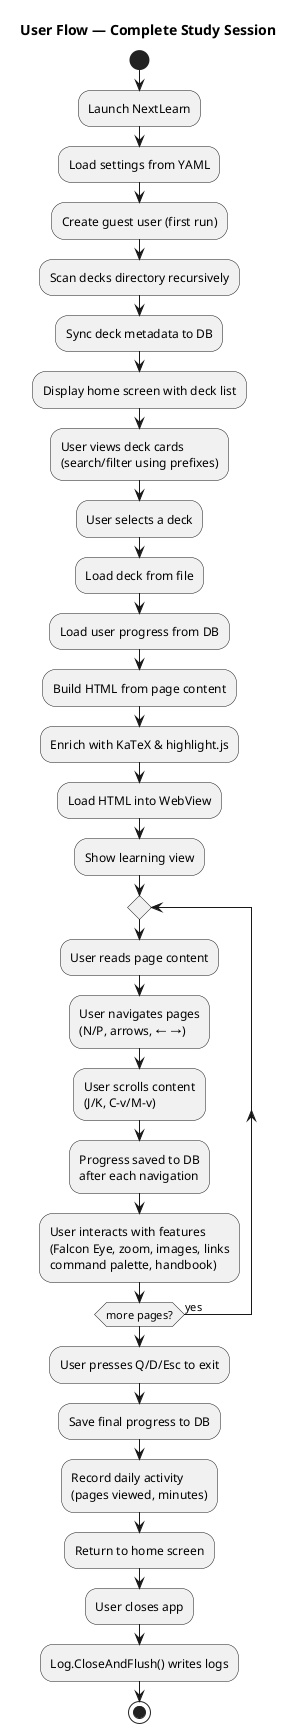
\includegraphics[height=700]{diagrams/flow-study.png}
\end{center}
\subsubsection{AI Feature Usage Flow}
\label{sec:orga721d28}
\begin{center}
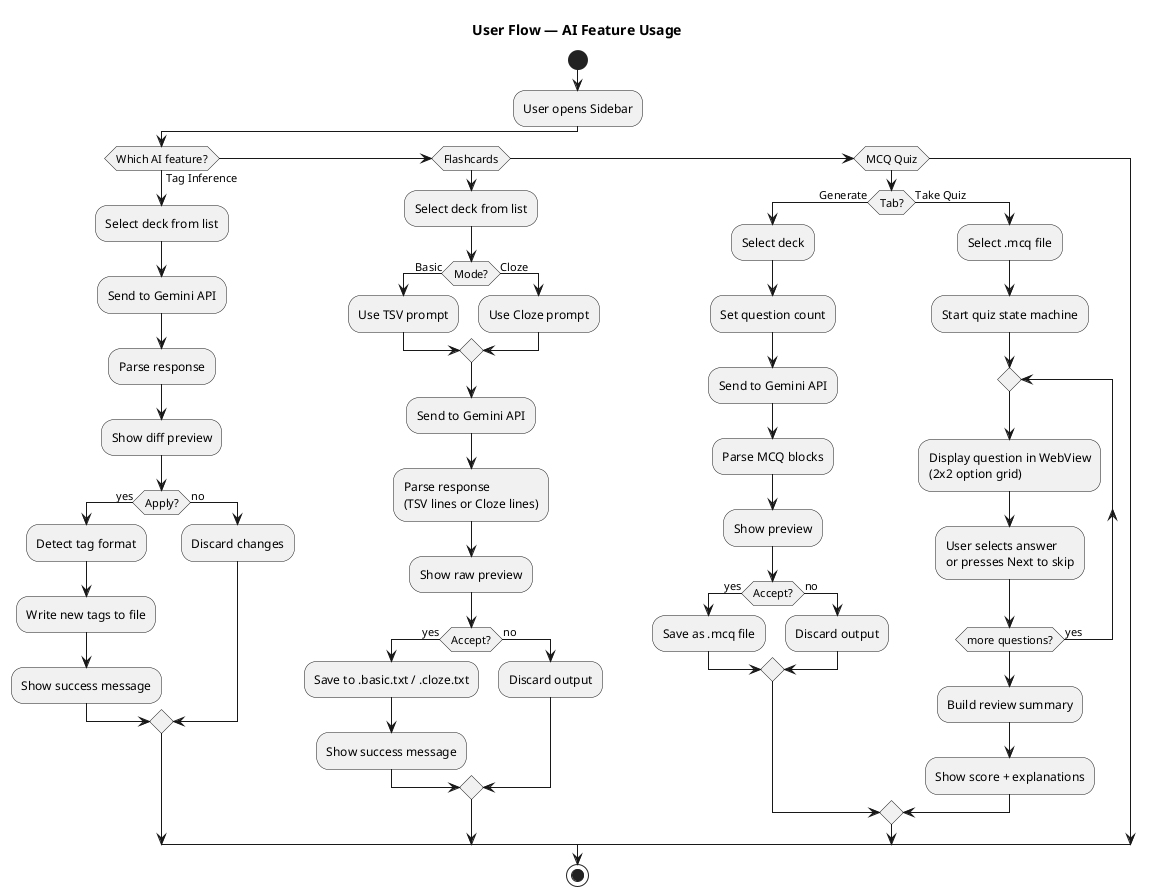
\includegraphics[width=.9\linewidth]{diagrams/flow-ai.png}
\end{center}
\subsection{Core Services}
\label{sec:org03409a9}
NextLearn is built around 21 key services, each with a specific
responsibility. Below is the complete inventory with roles and file
locations:
\subsubsection{services files}
\label{sec:org4a79992}
\begin{center}
\begin{tabular}{ll}
Service & File\\
\hline
ThemeHelper & Services/ThemeHelper.cs\\
DeckFileParser & Services/DeckFileParser.cs\\
DeckFileIdentity & Services/DeckFileIdentity.cs\\
DeckService & Services/DeckService.cs\\
DeckFileService & Services/DeckFileService.cs\\
UserService & Services/UserService.cs\\
SettingsService & Services/SettingsService.cs\\
HtmlContentBuilder & Services/HtmlContentBuilder.cs (1049 lines)\\
HtmlContentService & Services/HtmlContentService.cs\\
FalconEyeBuilder & Services/FalconEyeBuilder.cs\\
MarkdownInlineRenderer & Services/MarkdownInlineRenderer.cs\\
OrgInlineRenderer & Services/OrgInlineRenderer.cs\\
TagInferenceService & Services/TagInferenceService.cs\\
TagInferenceResult & Services/TagInferenceResult.cs\\
DeckFileWriter & Services/DeckFileWriter.cs\\
FlashcardService & Services/FlashcardService.cs\\
FlashcardGenerationMode & Services/FlashcardGenerationMode.cs\\
FlashcardResult & Services/FlashcardResult.cs\\
McqFileParser & Services/McqFileParser.cs\\
McqFileService & Services/McqFileService.cs\\
McqQuizHtmlBuilder & Services/McqQuizHtmlBuilder.cs\\
McqGenerationService & Services/McqGenerationService.cs\\
McqGenerationResult & Services/McqGenerationResult.cs\\
McqResultLogger & Services/McqResultLogger.cs\\
McqFileInfo & Services/McqFileInfo.cs\\
KeyBindingService & Services/KeyBindingService.cs (732 lines)\\
KeyboardHandler & Services/KeyboardHandler.cs\\
KeyboardActionKind & Services/KeyboardActionKind.cs\\
WebViewBridge & Services/WebViewBridge.cs\\
DeckFilter & Services/DeckFilter.cs\\
ViewLocator & ViewLocator.cs\\
\end{tabular}
\end{center}

\newpage
\subsubsection{what they do}
\label{sec:org2c00d15}
\begin{center}
\begin{tabular}{ll}
Service & Role\\
\hline
ThemeHelper & Runtime dark/light color dictionaries, live ApplyTheme()\\
DeckFileParser & Static parser: frontmatter + heading → Deck+Pages\\
DeckFileIdentity & SHA256 of path → deterministic GUID\\
DeckService & DB layer: CRUD for decks, pages, progress\\
DeckFileService & File ops: archive/pin/rename (no DB dependency)\\
UserService & Guest user creation, streak computation, daily activity recording\\
SettingsService & YAML persistence for theme/font/paths/API key/keybindings\\
HtmlContentBuilder & Static HTML builder from Page model (markdown/org → HTML)\\
HtmlContentService & HTML enrichment with KaTeX, highlight.js, copy buttons\\
FalconEyeBuilder & Table-of-contents HTML generation from Deck headings\\
MarkdownInlineRenderer & Strategy for .md inline rendering (bold, italic, code, links)\\
OrgInlineRenderer & Strategy for .org inline rendering (same constructs + org syntax)\\
TagInferenceService & Gemini API client: model discovery, retry, tag parsing (435 lines)\\
TagInferenceResult & AI tag suggestion result DTO\\
DeckFileWriter & Tag write-back (7 formats) + frontmatter health check\\
FlashcardService & Gemini API client: basic+cloze generation, mode-aware parsing\\
FlashcardGenerationMode & Enum: Basic / Cloze\\
FlashcardResult & AI flashcard generation result DTO\\
McqFileParser & Parse/serialize .mcq files (YAML frontmatter + question blocks)\\
McqFileService & List/read/delete .mcq files\\
McqQuizHtmlBuilder & Interactive quiz HTML (2×2 grid, timer, scoring, review)\\
McqGenerationService & Gemini API client for MCQ generation\\
McqGenerationResult & MCQ generation result DTO\\
McqResultLogger & Logs quiz results to .mcq.result files\\
McqFileInfo & MCQ file metadata DTO\\
KeyBindingService & Keyboard profiles: Vim/Emacs/VS Code/Custom; binding definitions\\
KeyboardHandler & Routes key events to actions by context + profile\\
KeyboardActionKind & Enum: 67 possible keyboard actions\\
WebViewBridge & native communication (key bridge, URI interception, image overlay)\\
DeckFilter & Search tokenizer with \url{file:///title:/desc:/tags}: prefixes\\
ViewLocator & ViewModel→View resolution via naming convention\\
\end{tabular}
\end{center}


\newpage
\section{Testing Strategy}
\label{sec:org3168b1e}
\subsection{Unit Test Framework}
\label{sec:org596be0c}
NextLearn uses xUnit as the test framework with FluentAssertions for
readable assertions and NSubstitute for mocking.

Test project location: \texttt{tests/NextLearn.Desktop.Tests/}
\subsection{Test Files}
\label{sec:orgaa621d7}
\begin{center}
\begin{tabular}{lll}
Test File & Lines & Scope\\
\hline
DeckFileParserTests.cs & \textasciitilde{}200 & .md/.org/.txt parsing, frontmatter, headings\\
DeckFileServiceTests.cs & \textasciitilde{}150 & Pin/archive/rename file ops, subdirectory\\
DeckServiceTests.cs & 472 & DB CRUD, progress tracking, metadata sync\\
EdgeCaseTests.cs & 223 & Empty files, special chars, cross-format edge\\
HtmlContentBuilderTests.cs & \textasciitilde{}200 & HTML output, inline rendering, wiki-link detection\\
SettingsServiceTests.cs & 139 & YAML load/save, path resolution, defaults\\
UserServiceTests.cs & \textasciitilde{}200 & User creation, streak computation, daily activity\\
\end{tabular}
\end{center}
\subsection{Test Approach}
\label{sec:org82bab71}
\begin{itemize}
\item \textbf{\textbf{Repository pattern for DB}}: Entity Framework Core InMemory provider
for database tests — no real SQLite dependency.
\item \textbf{\textbf{File system isolation}}: DeckFileServiceTests use temporary
directories created and cleaned per test.
\item \textbf{\textbf{Mocked HTTP}}: TagInferenceService, FlashcardService, and
McqGenerationService tests use mocked HttpClient handlers to avoid
real API calls.
\item \textbf{\textbf{Round-trip testing}}: Parser tests follow parse→serialize→re-parse
cycles with assertion of equivalence.
\item \textbf{\textbf{Edge case tables}}: plan-todos.org contains exhaustive edge case
tables for every AI feature, with each case tested.
\end{itemize}
\subsection{CI/CD Pipeline}
\label{sec:org3bd70f8}
GitHub Actions (\texttt{.github/workflows/ci.yml}) runs on every push:

\begin{verbatim}
Trigger: push to any branch
Matrix: ubuntu-latest, windows-latest, macos-latest

Steps:
  1. Checkout repository
  2. Setup .NET 10.0 SDK
  3. dotnet restore
  4. dotnet build (TreatWarningsAsErrors enforced)
  5. dotnet test (all platforms)
  6. dotnet publish (single-file self-contained)
     - linux-x64
     - osx-arm64
     - win-x64
  7. Upload artifacts
\end{verbatim}

\newpage
\section{UI/UX Design}
\label{sec:org1225fe6}
\subsection{Logo \& Branding}
\label{sec:org1baf76d}
\begin{center}

\includegraphics[width=200]{./screenshots/nextlearn-logo-high-res.png}
\end{center}

The NextLearn logo features a stylized brain/network motif in purple
gradient (\#7C0AED primary). The design communicates:
\begin{itemize}
\item Neural connections (learning)
\item Structured thinking (network graph)
\item Modern, minimalist aesthetic
\end{itemize}

The application icon is rendered in the title bar and used as the
application launcher icon (installed via \texttt{install-icon.sh} on Linux).
\subsection{Screenshot Showcase}
\label{sec:org5d14074}
\subsubsection{Home \& Navigation}
\label{sec:org3c53b09}
\begin{center}
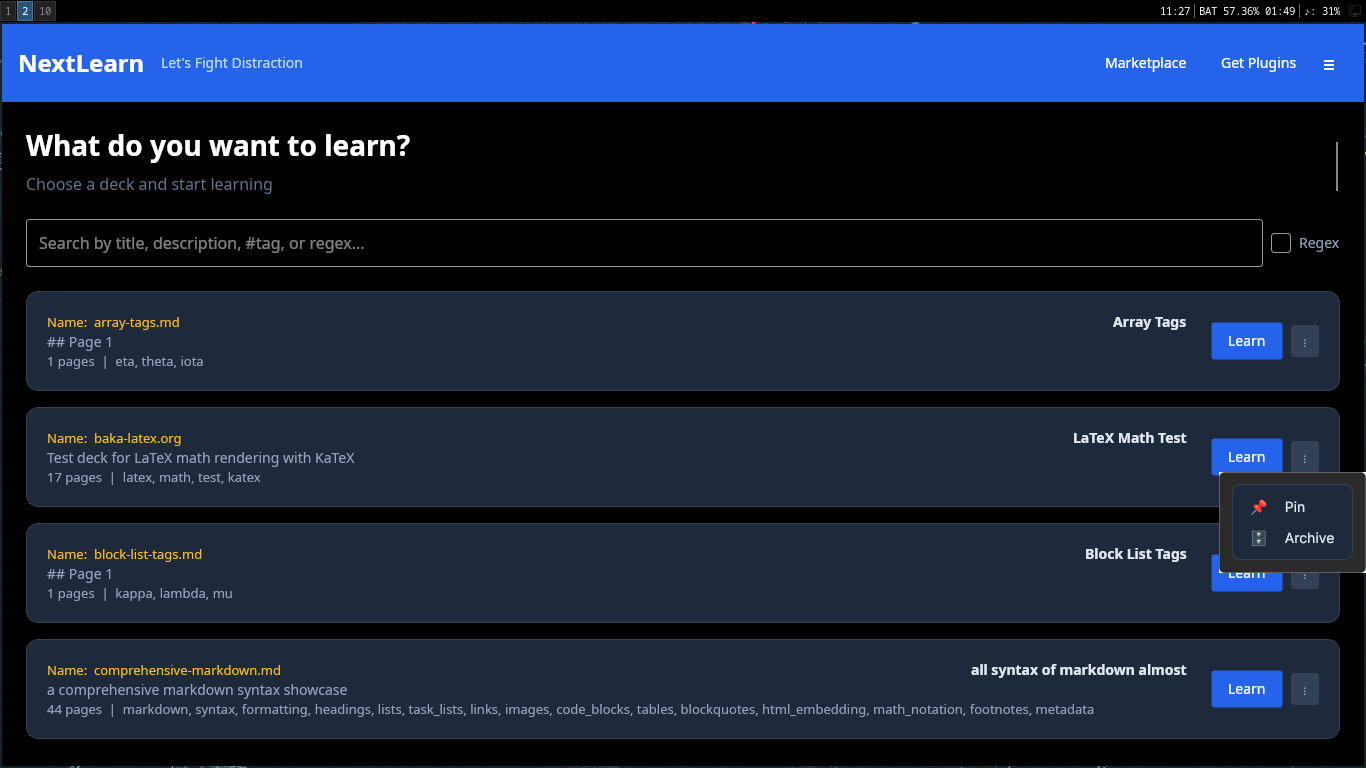
\includegraphics[width=550]{./screenshots/home-search-page.png}
\end{center}

\textbf{Figure 1: Home page with search bar, showing filtered deck list.}

\begin{center}
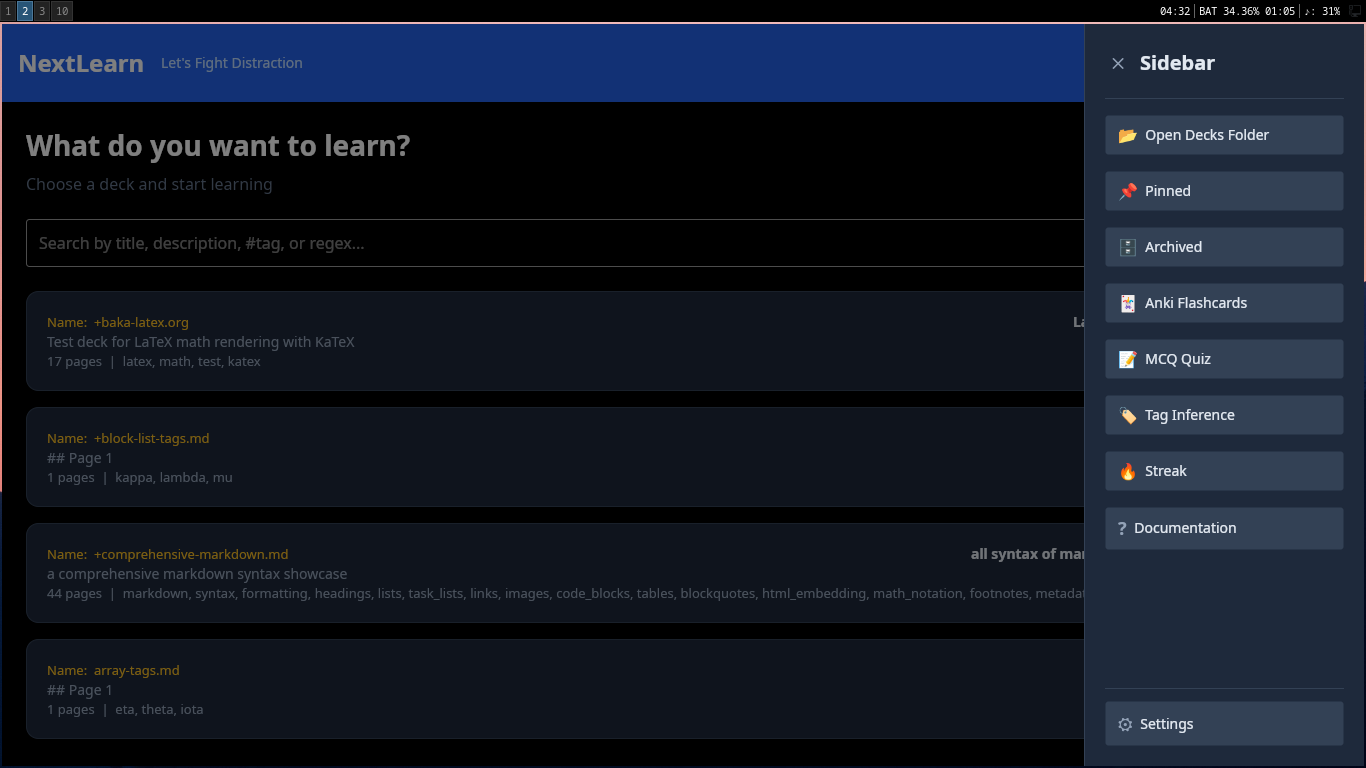
\includegraphics[width=550]{./screenshots/sidebar-panel.png}
\end{center}

\textbf{Figure 2: Sidebar panel with navigation links and settings.}

\begin{center}
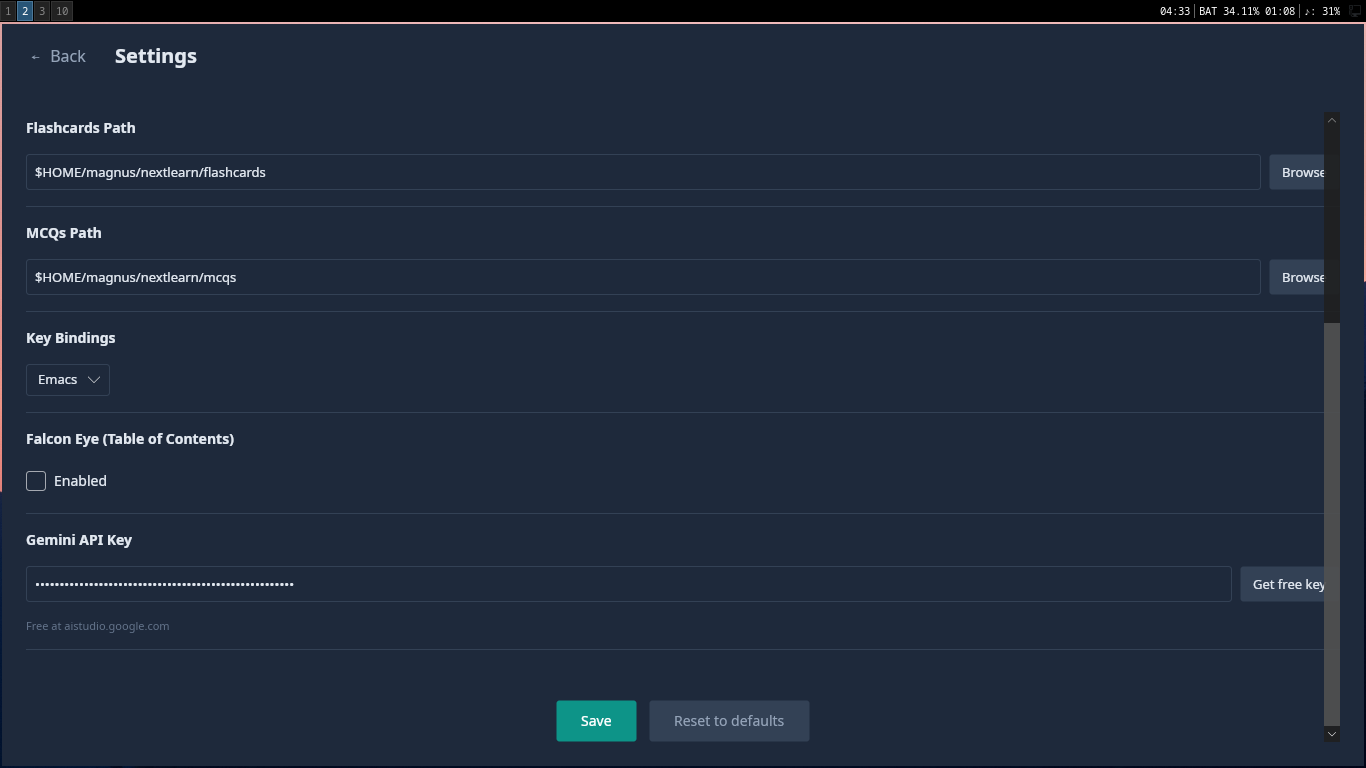
\includegraphics[width=550]{./screenshots/settings-panel.png}
\end{center}

\textbf{Figure 3: Settings page — theme, font, paths, keybinding profile, Gemini API key.}

\begin{center}
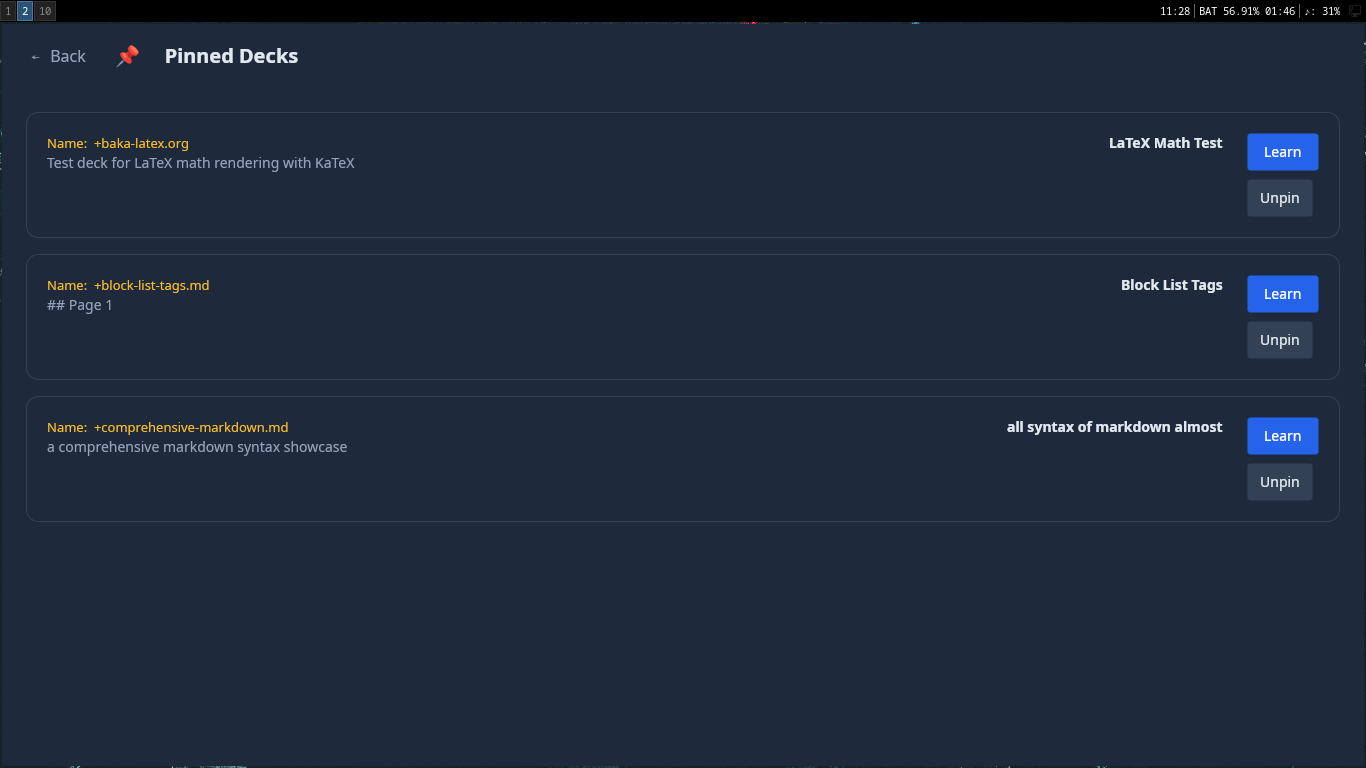
\includegraphics[width=550]{./screenshots/pinned-panel.png}
\end{center}

\textbf{Figure 4: Pinned decks overlay for quick access to favorite decks.}

\begin{center}
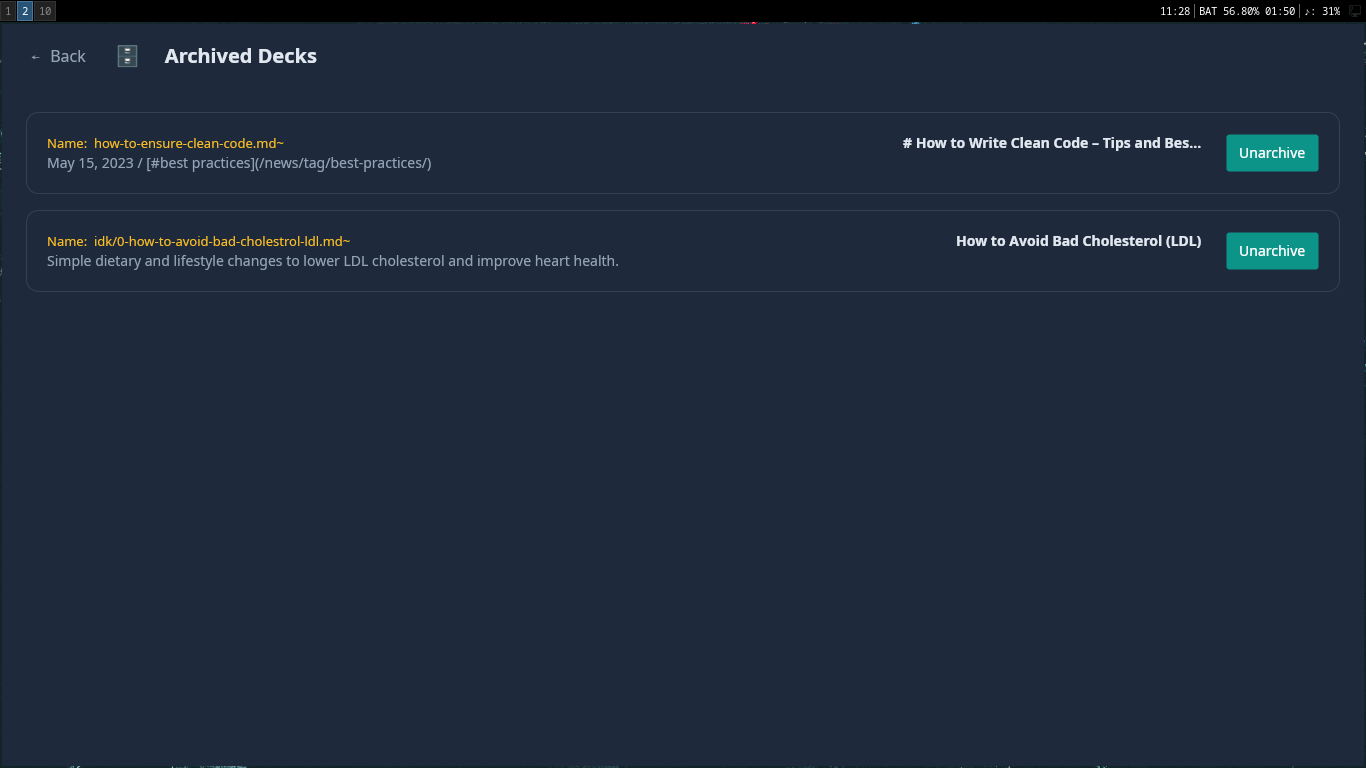
\includegraphics[width=550]{./screenshots/archived-panel.png}
\end{center}

\textbf{Figure 5: Archived decks overlay.}

\begin{center}
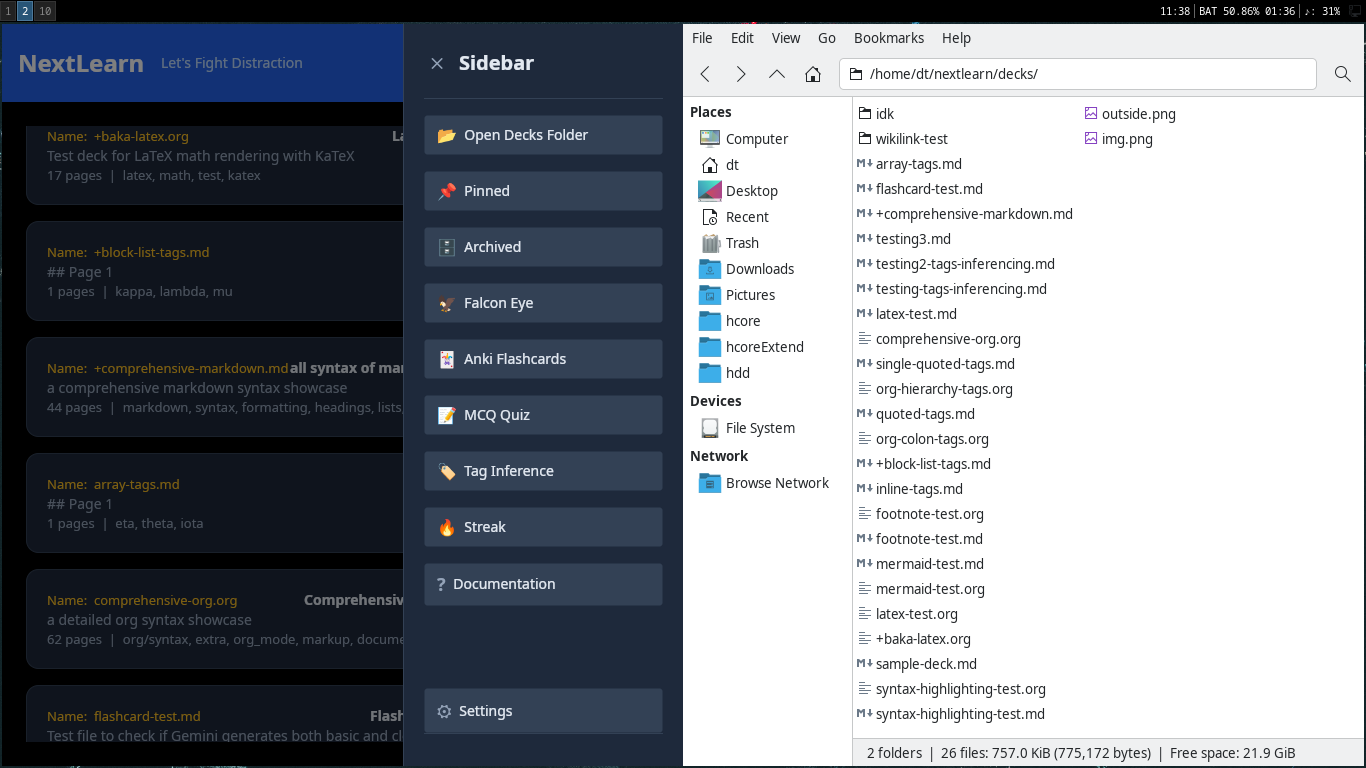
\includegraphics[width=550]{./screenshots/open-decks-directory-feature.png}
\end{center}

\textbf{Figure 6: Open decks folder in system file manager.}

\begin{center}
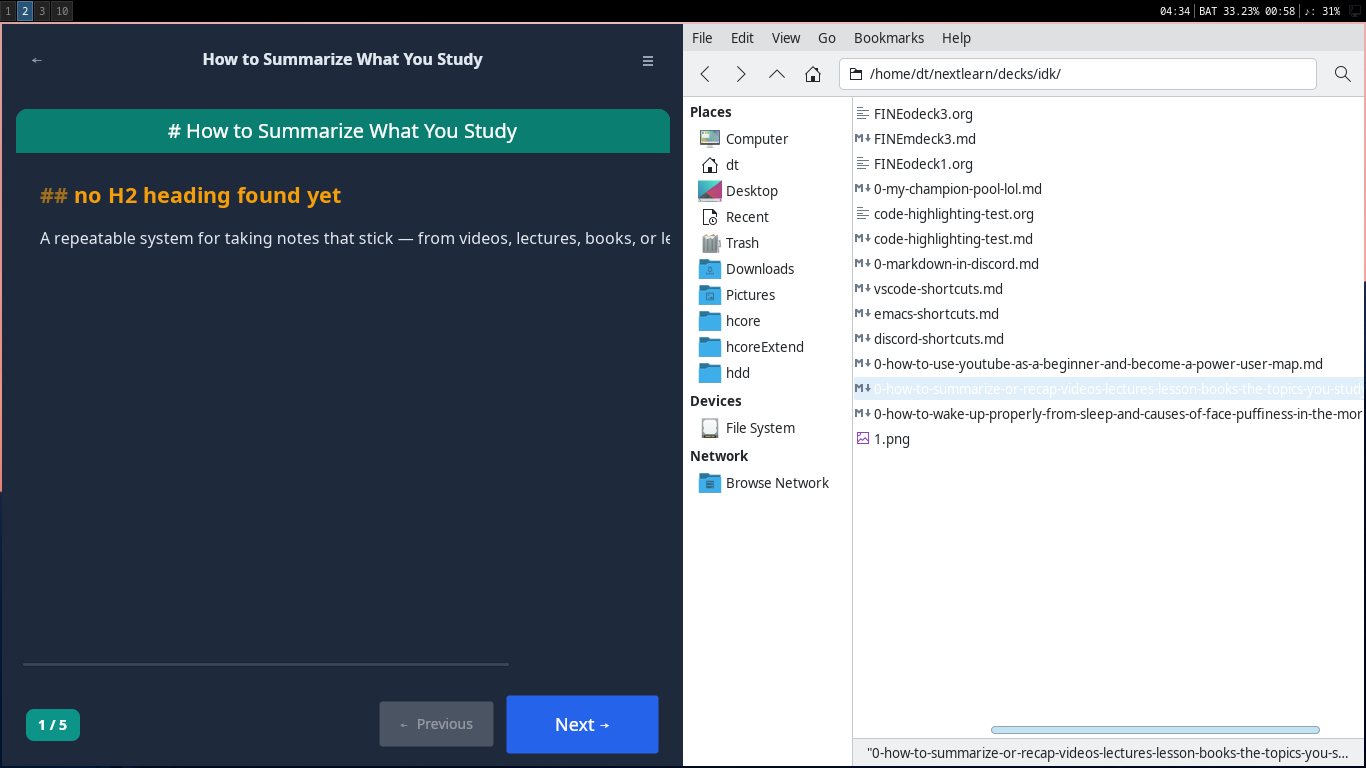
\includegraphics[width=550]{./screenshots/reveal-deck-feature.png}
\end{center}

\textbf{Figure 7: Reveal current deck file in file manager.}
\subsubsection{Study Page}
\label{sec:org3b63e5a}
\begin{center}
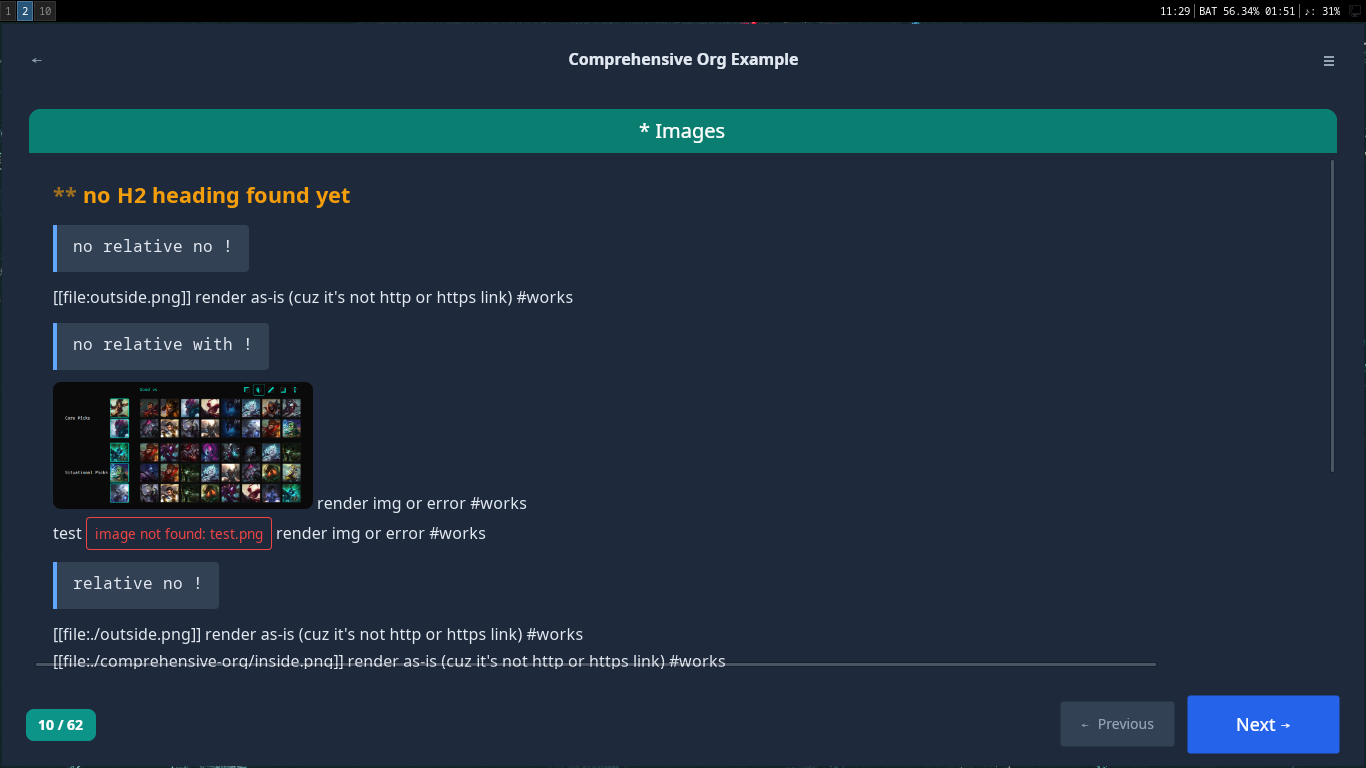
\includegraphics[width=550]{./screenshots/study-page.png}
\end{center}

\textbf{Figure 8: Main study view with deck loaded — page content, page counter,
section breadcrumbs.}

\begin{center}
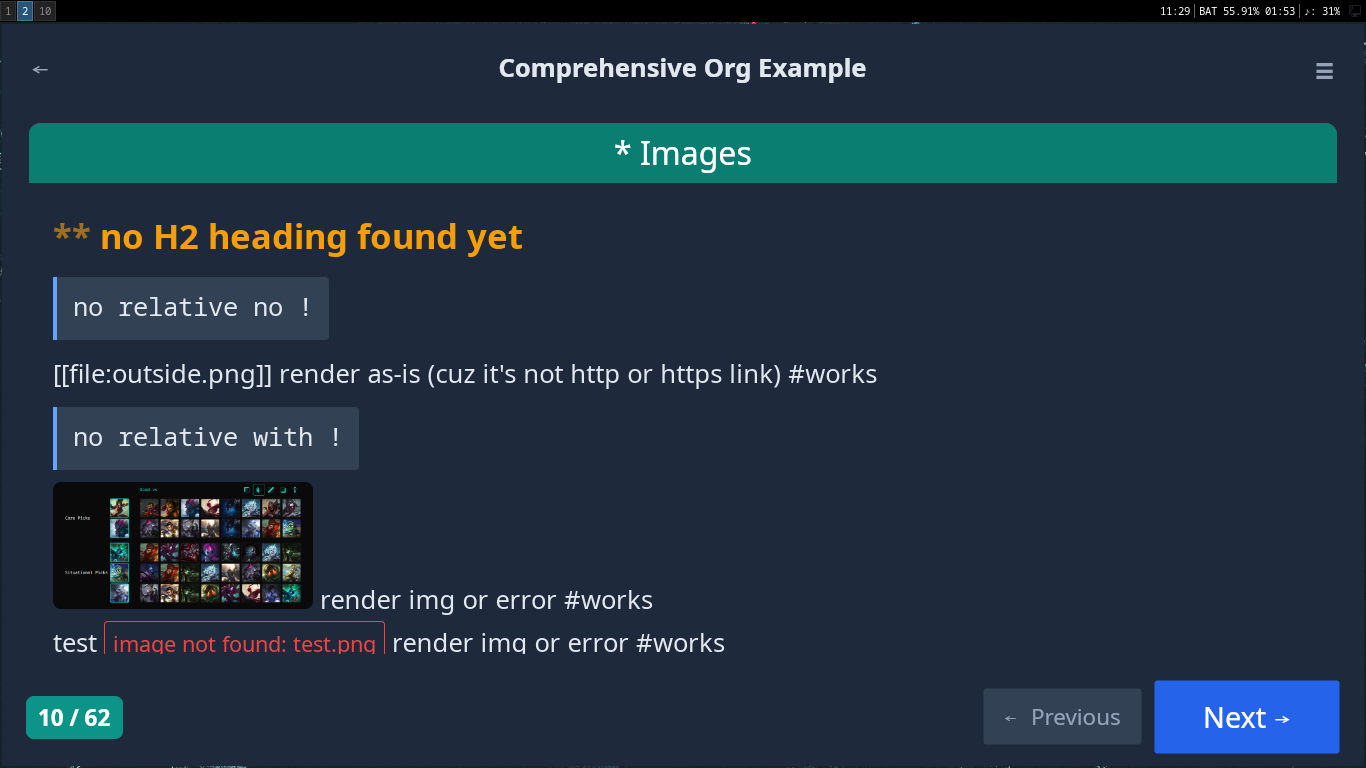
\includegraphics[width=550]{./screenshots/zoom-in-text.png}
\end{center}

\textbf{Figure 9: Text zoomed in via Ctrl+Shift++.}

\begin{center}
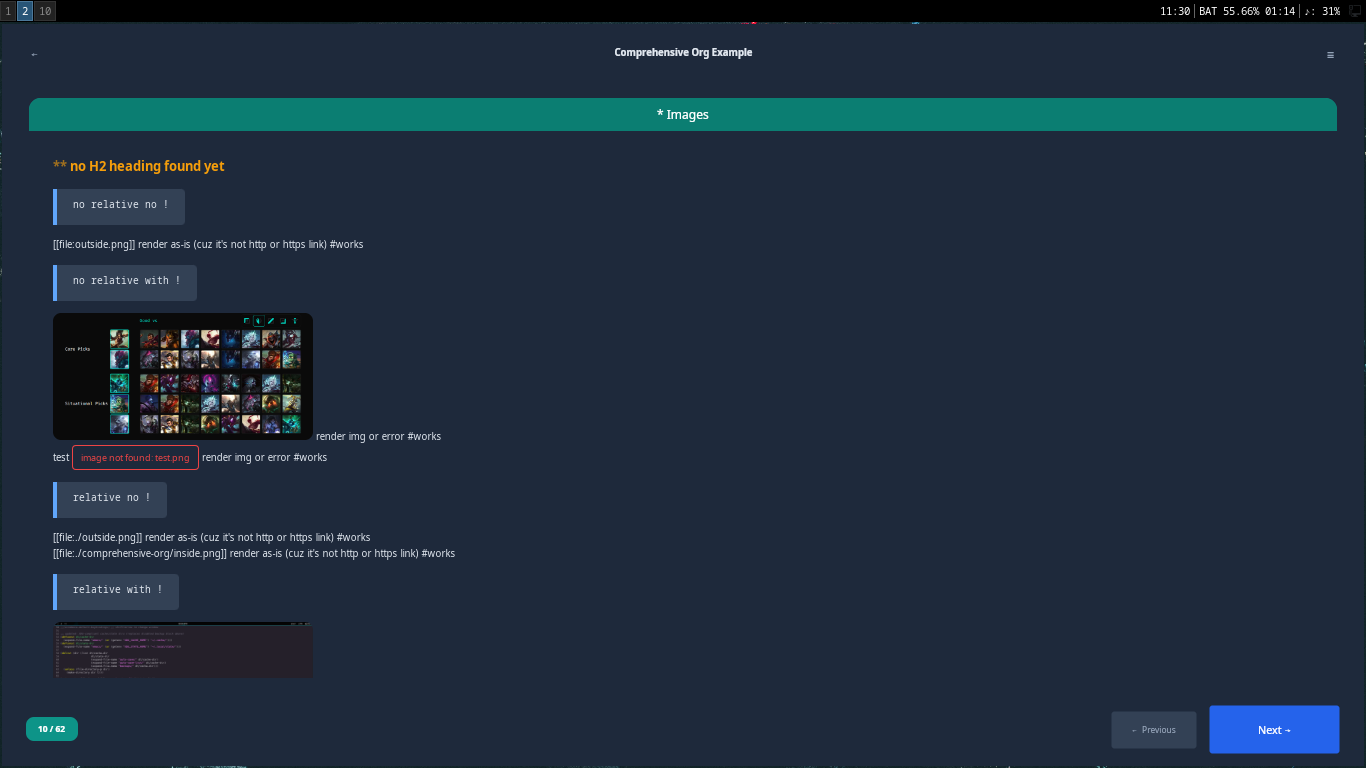
\includegraphics[width=550]{./screenshots/zoom-out-text.png}
\end{center}

\textbf{Figure 10: Text zoomed out via Ctrl+Shift+-.}
\subsubsection{Command Palette \& Handbook}
\label{sec:orgbf5c1c4}
\begin{center}
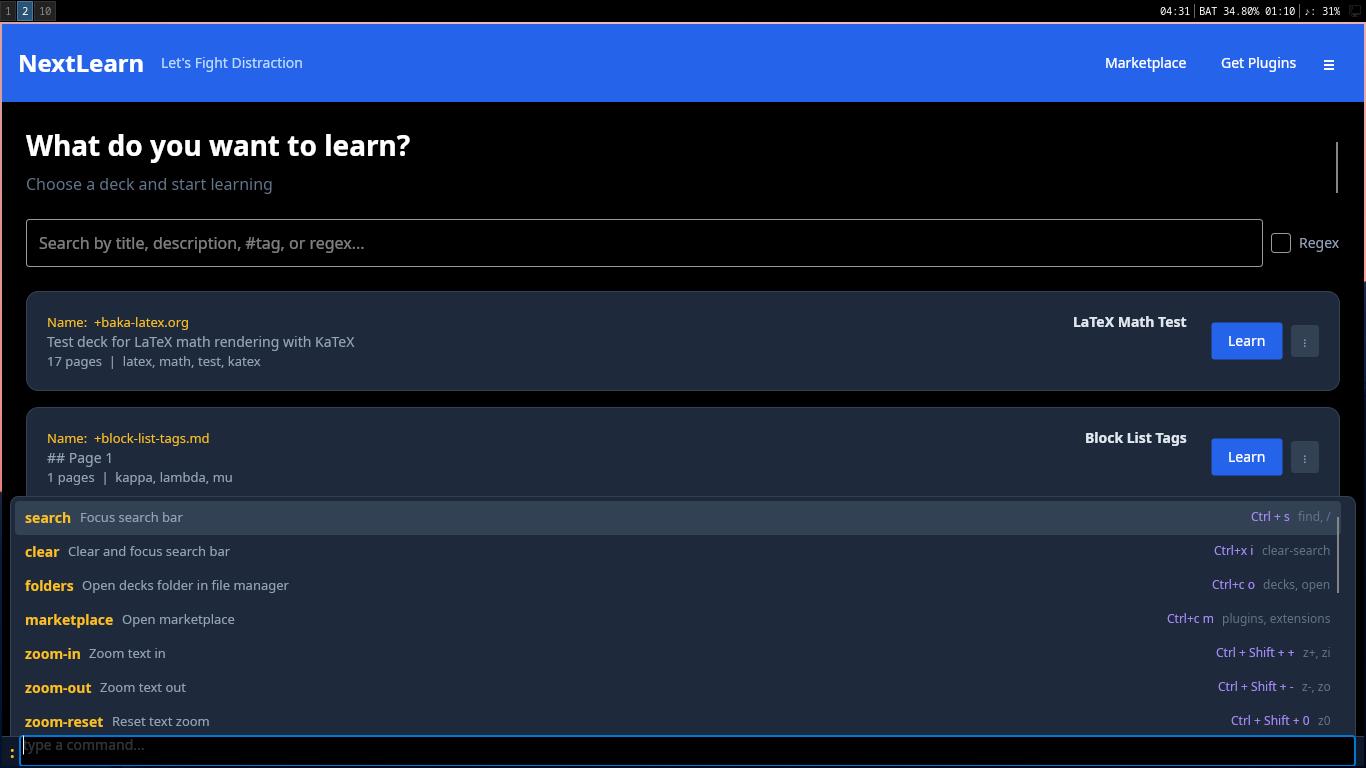
\includegraphics[width=550]{./screenshots/cmd-palette-feature.png}
\end{center}

\textbf{Figure 11: Command palette for quick action lookup.}

\begin{center}
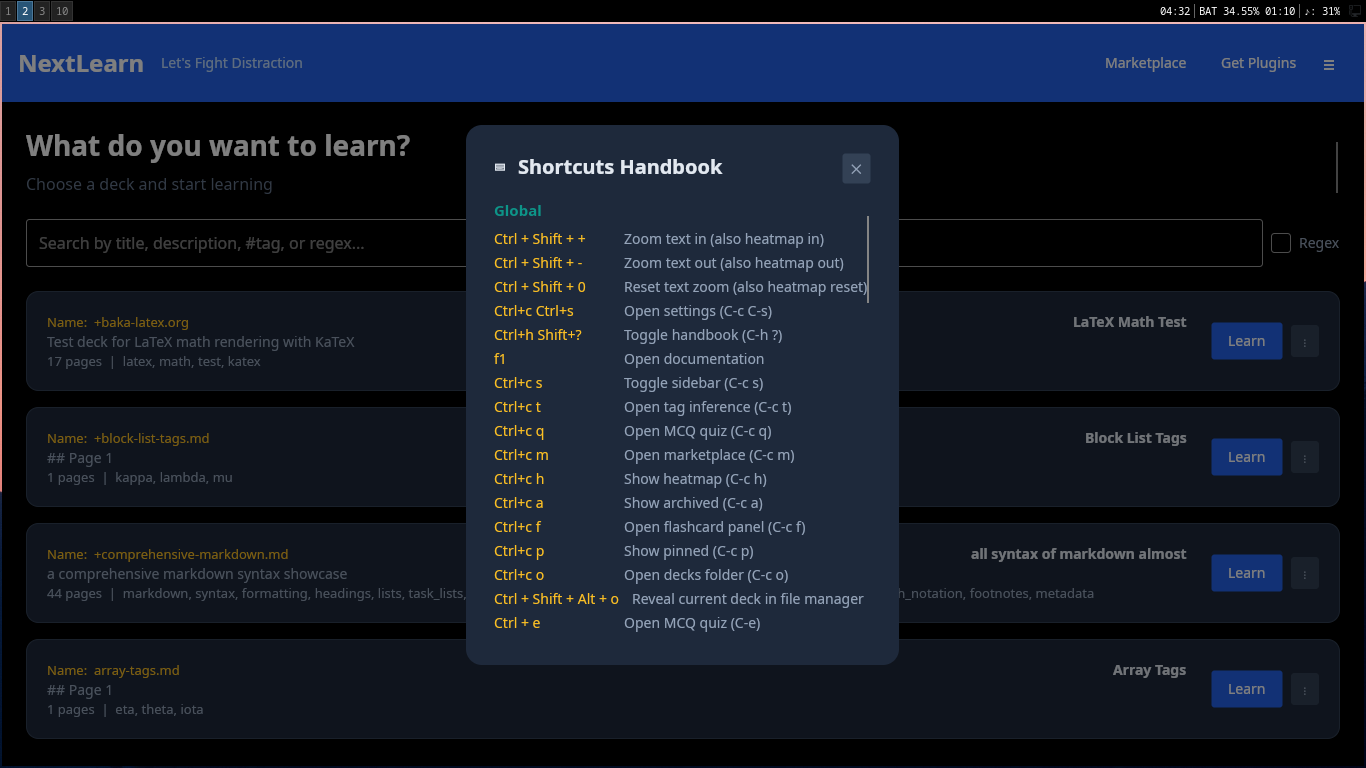
\includegraphics[width=550]{./screenshots/shortcuts-handbook-feature.png}
\end{center}

\textbf{Figure 12: Shortcuts handbook, auto-generated from current keybinding profile.}
\subsubsection{Falcon Eye (TOC)}
\label{sec:org654848e}
\begin{center}
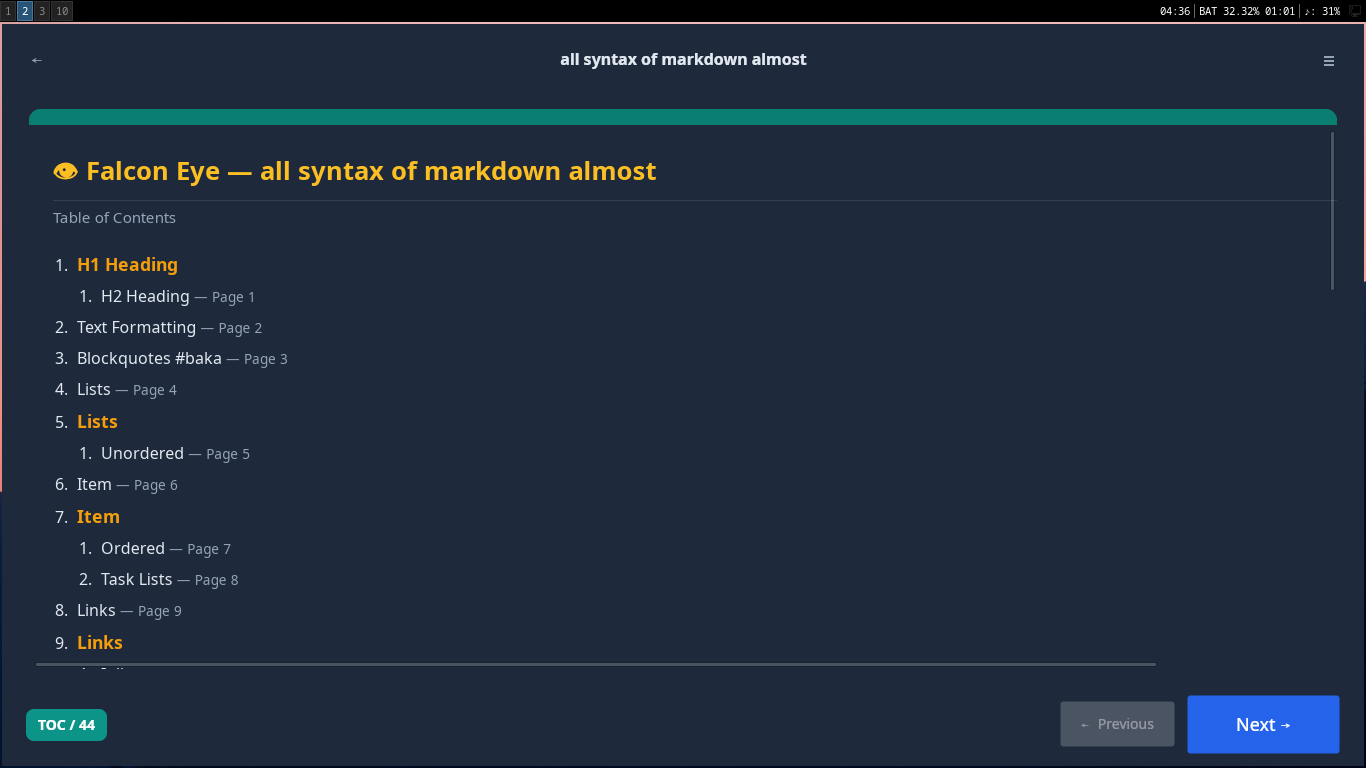
\includegraphics[width=550]{./screenshots/falcon-eye-feature.png}
\end{center}

\textbf{Figure 13: Falcon Eye table of contents — clickable entries navigate to
exact page.}
\subsubsection{Image Overlay}
\label{sec:org0696f38}
\begin{center}
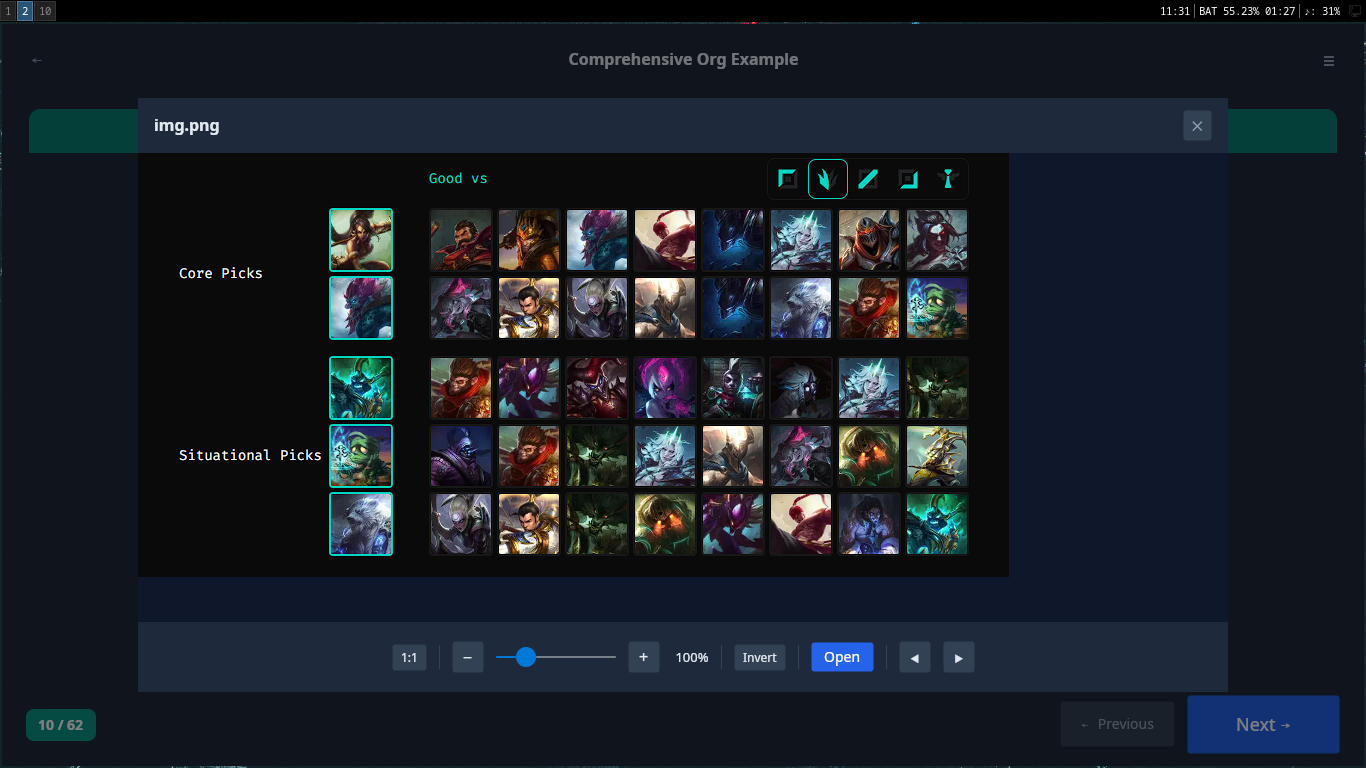
\includegraphics[width=550]{./screenshots/image-overlay-feature.png}
\end{center}

\textbf{Figure 14: Image overlay with navigation, zoom slider, and toolbar.}

\begin{center}
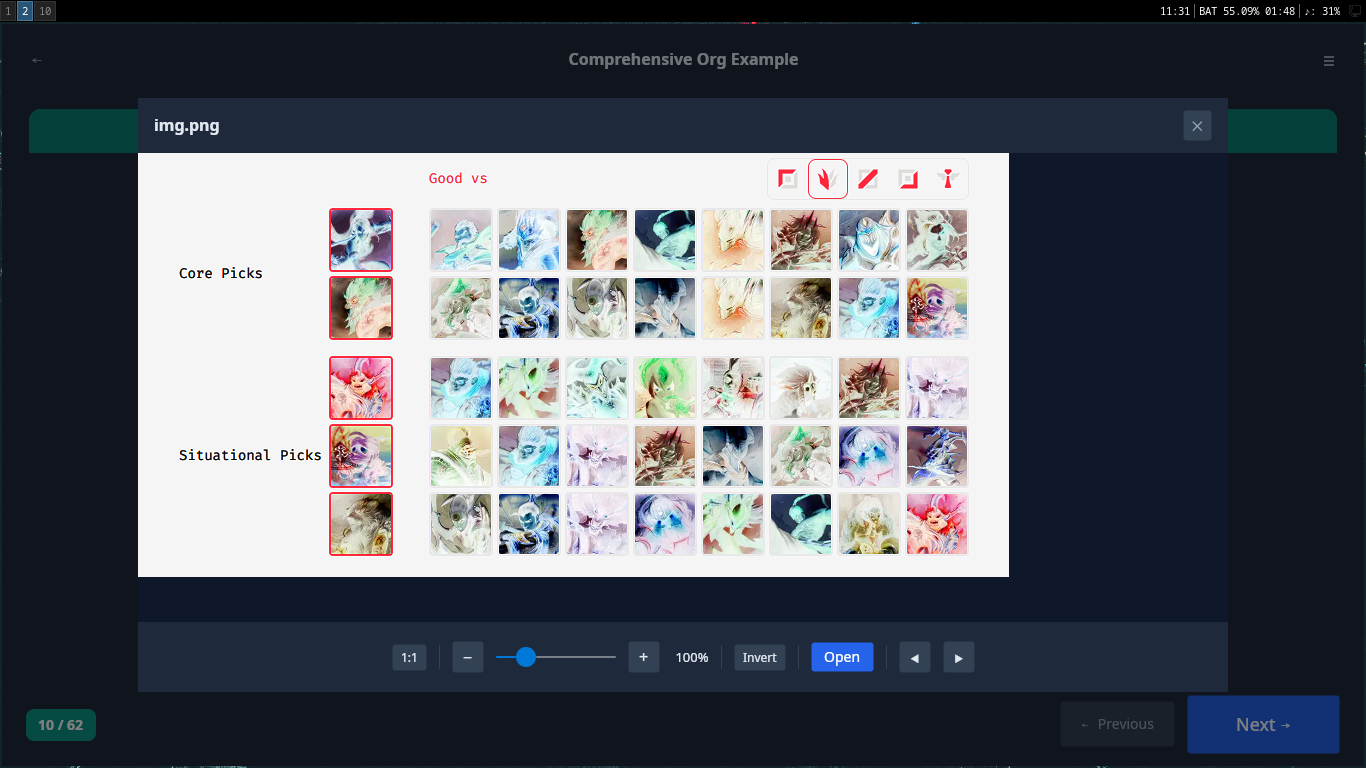
\includegraphics[width=550]{./screenshots/image-overlay-invert-colors.png}
\end{center}

\textbf{Figure 15: Image overlay with inverted colors for dark mode readability.}
\subsubsection{Heatmap \& Streaks}
\label{sec:org4e92edd}
\begin{center}
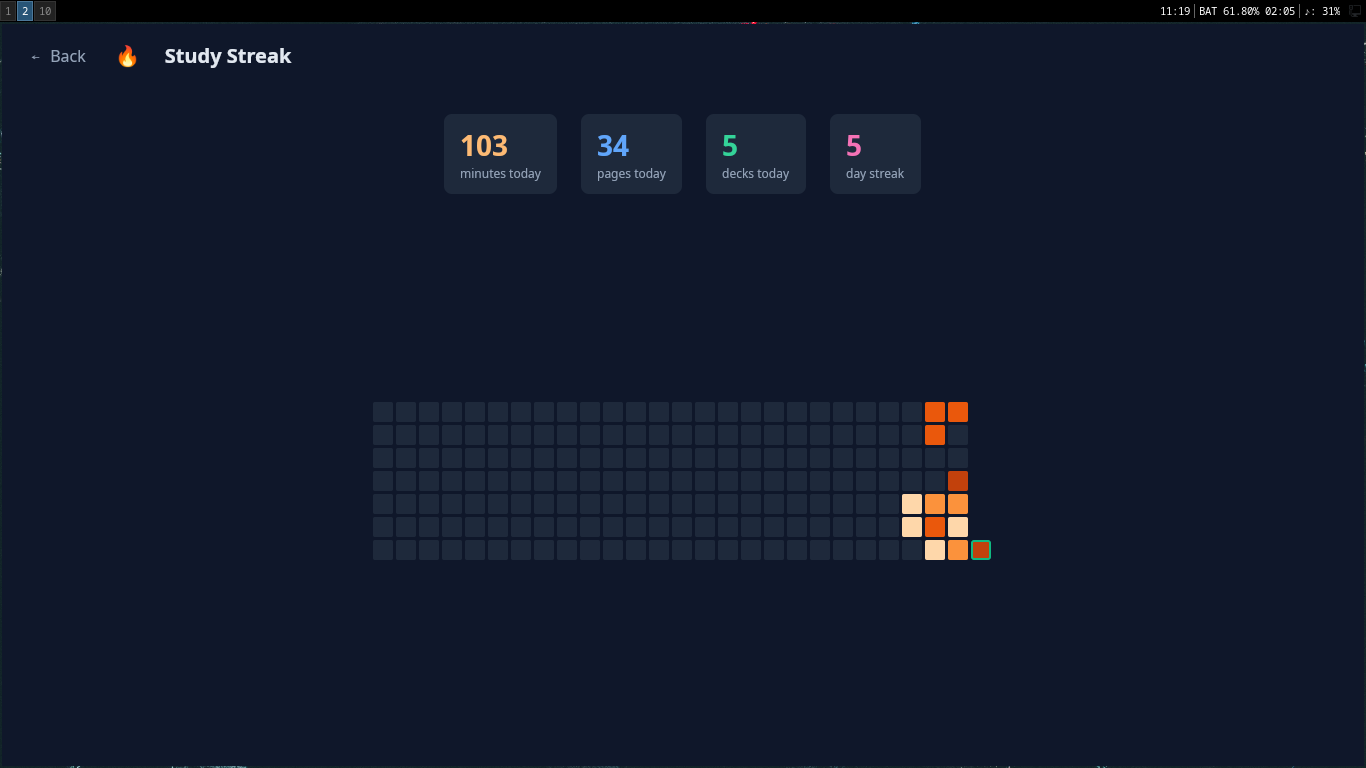
\includegraphics[width=550]{./screenshots/heatmap-streak-panel.png}
\end{center}

\textbf{Figure 16: Study streak heatmap — snake layout, 6-level orange scale,
green for today.}
\subsubsection{Tag Inference}
\label{sec:org6869fa9}
\begin{center}
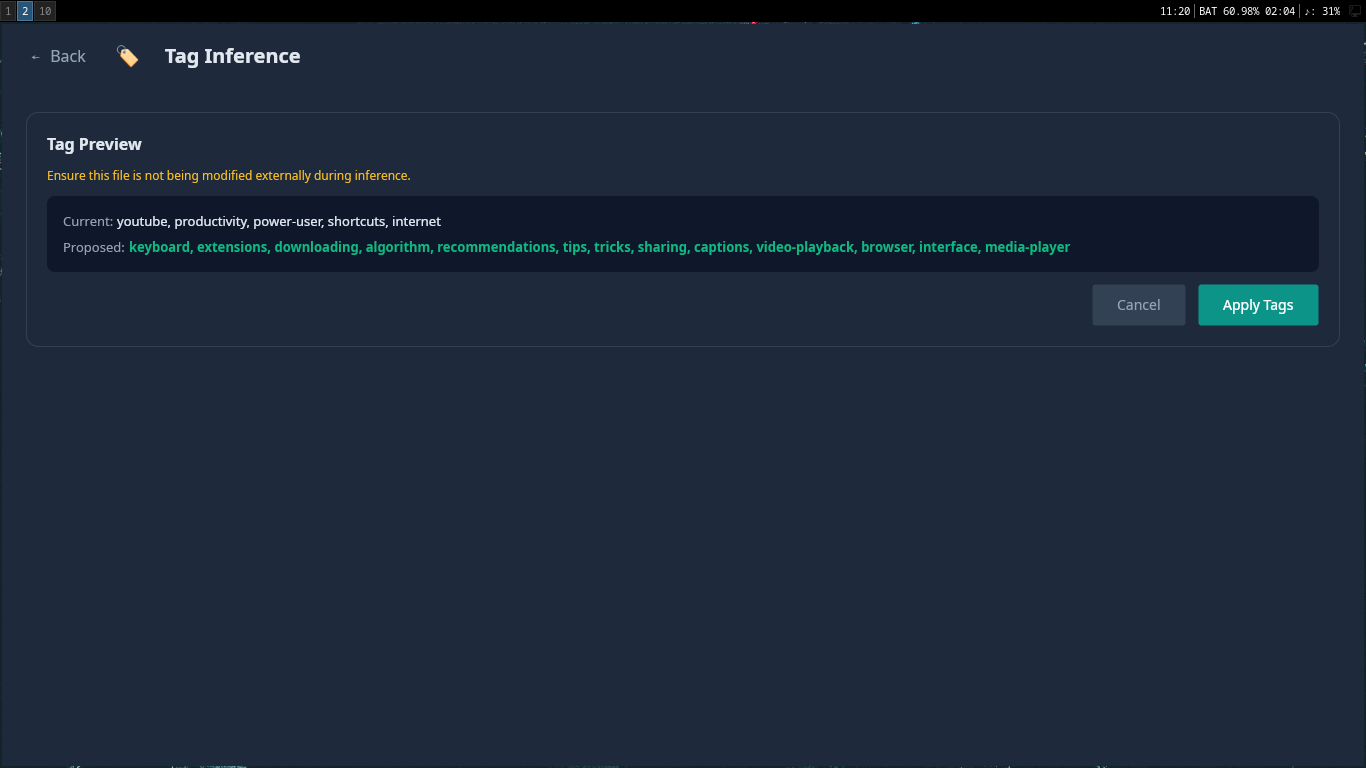
\includegraphics[width=550]{./screenshots/tags-inferencing-panel.png}
\end{center}

\textbf{Figure 17: AI tag inference panel using Google Gemini — select deck,
diff preview, apply with one click.}
\subsubsection{Flashcard Generation}
\label{sec:org7518c8c}
\begin{center}
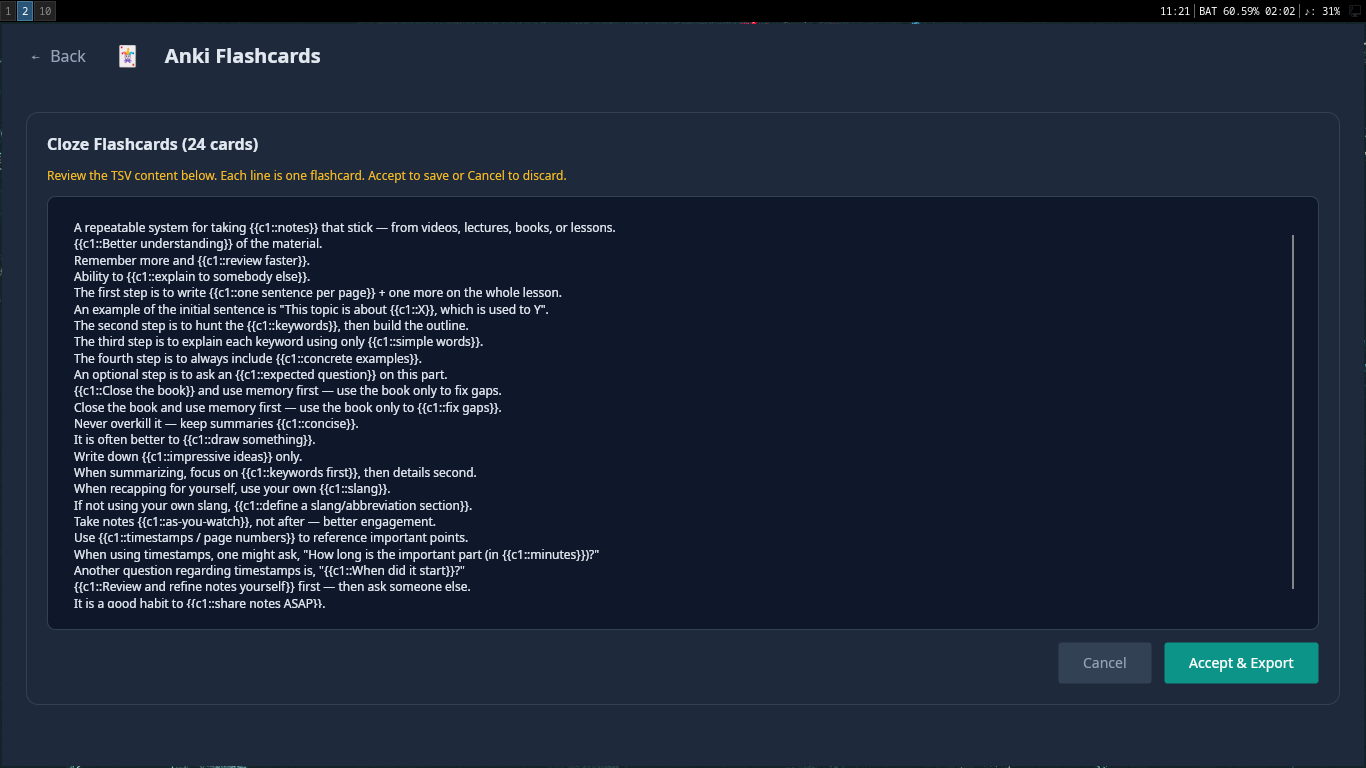
\includegraphics[width=550]{./screenshots/anki-flashcards-generation-panel.png}
\end{center}

\textbf{Figure 18: Anki flashcard generation panel — Basic and Cloze modes.}
\subsubsection{MCQ Quiz}
\label{sec:org5df4aed}
\begin{center}
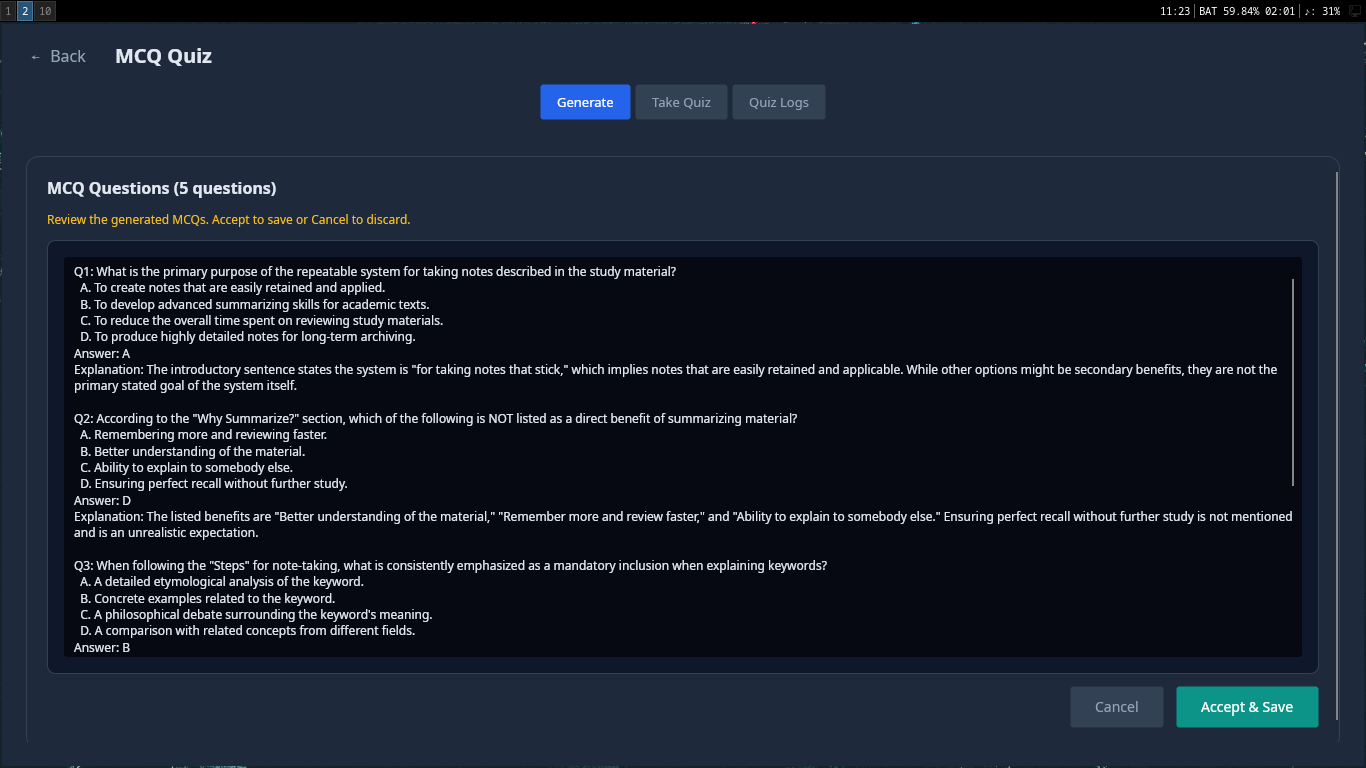
\includegraphics[width=550]{./screenshots/mcq-generate-tab.png}
\end{center}

\textbf{Figure 19: MCQ quiz generate tab — configure and generate via Gemini.}

\begin{center}
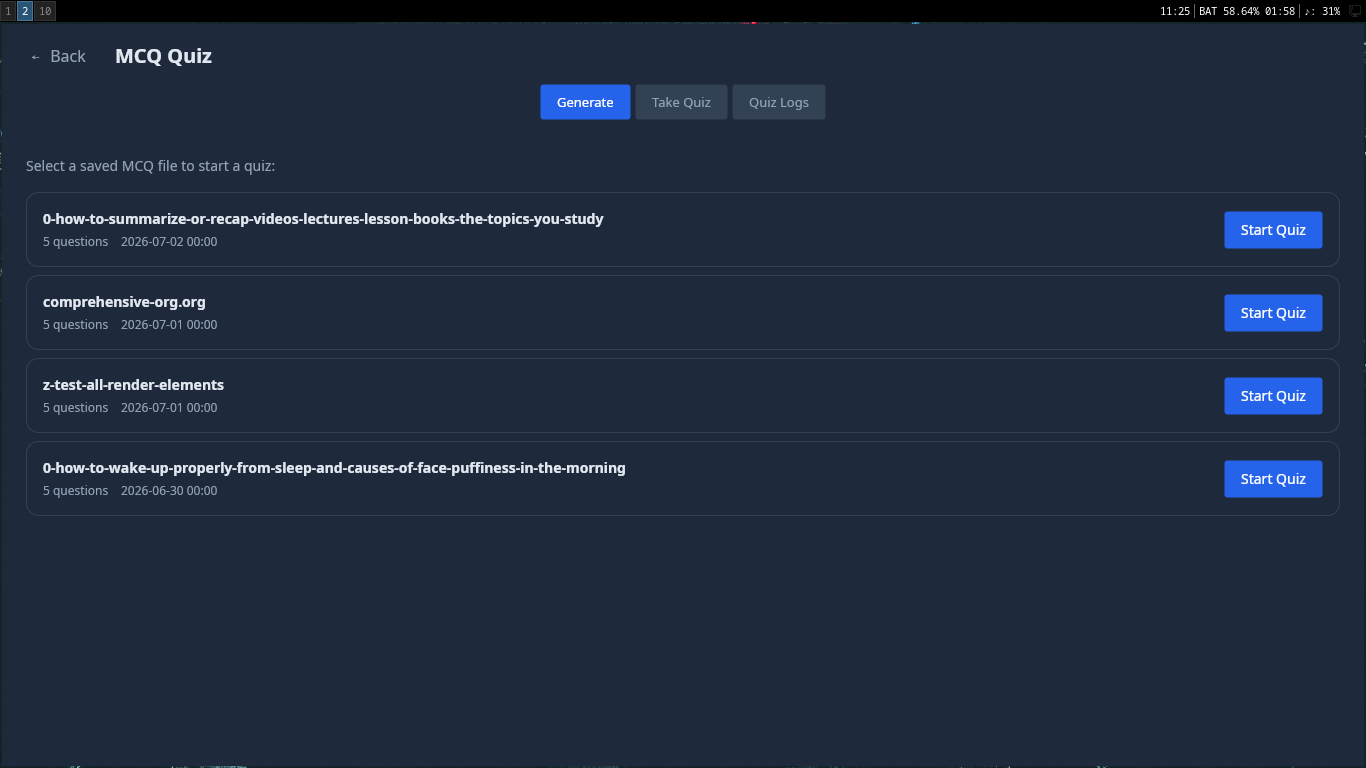
\includegraphics[width=550]{./screenshots/mcq-take-quiz-tab.png}
\end{center}

\textbf{Figure 20: MCQ quiz take tab — select a quiz and start interactive session.}

\begin{center}
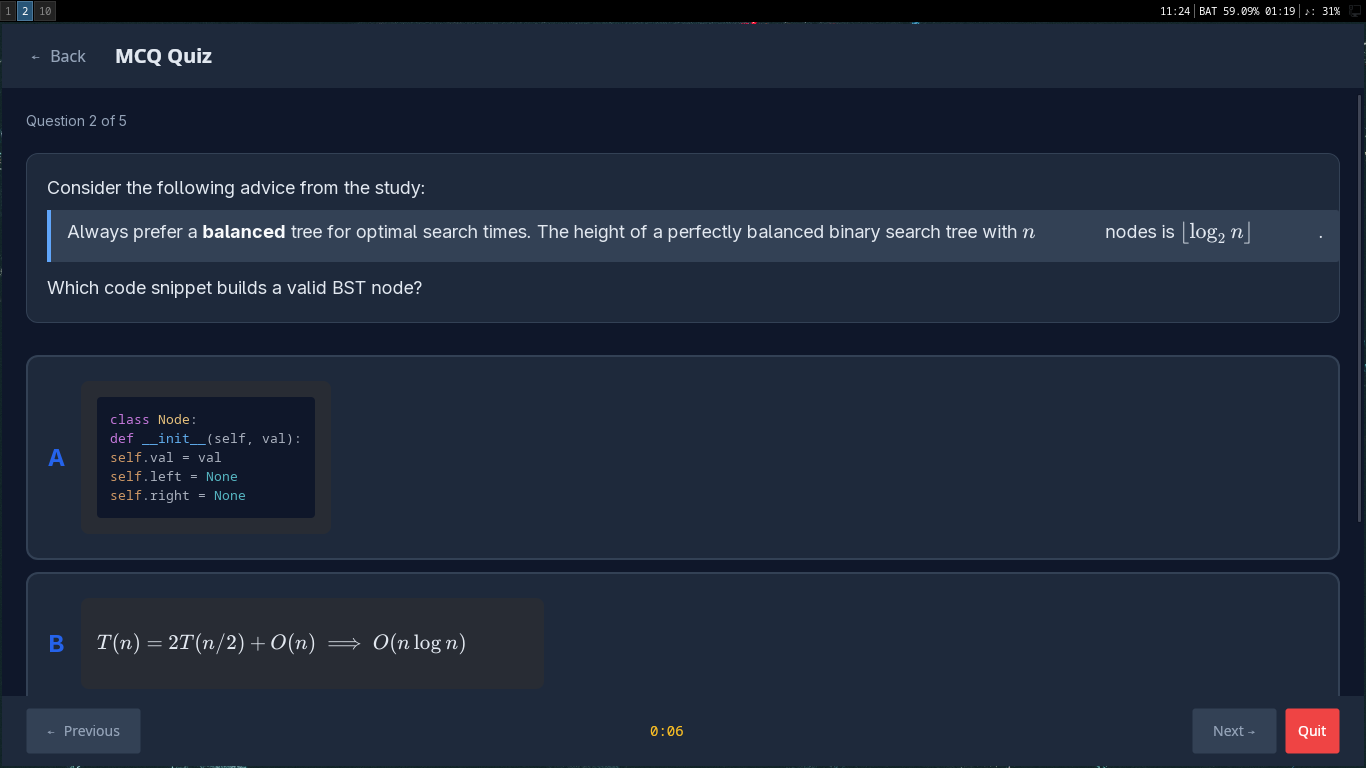
\includegraphics[width=550]{./screenshots/mcq-interactive-quiz-ui.png}
\end{center}

\textbf{Figure 21: Interactive MCQ quiz WebView — 4 item list, scoring, timer.}

\begin{center}
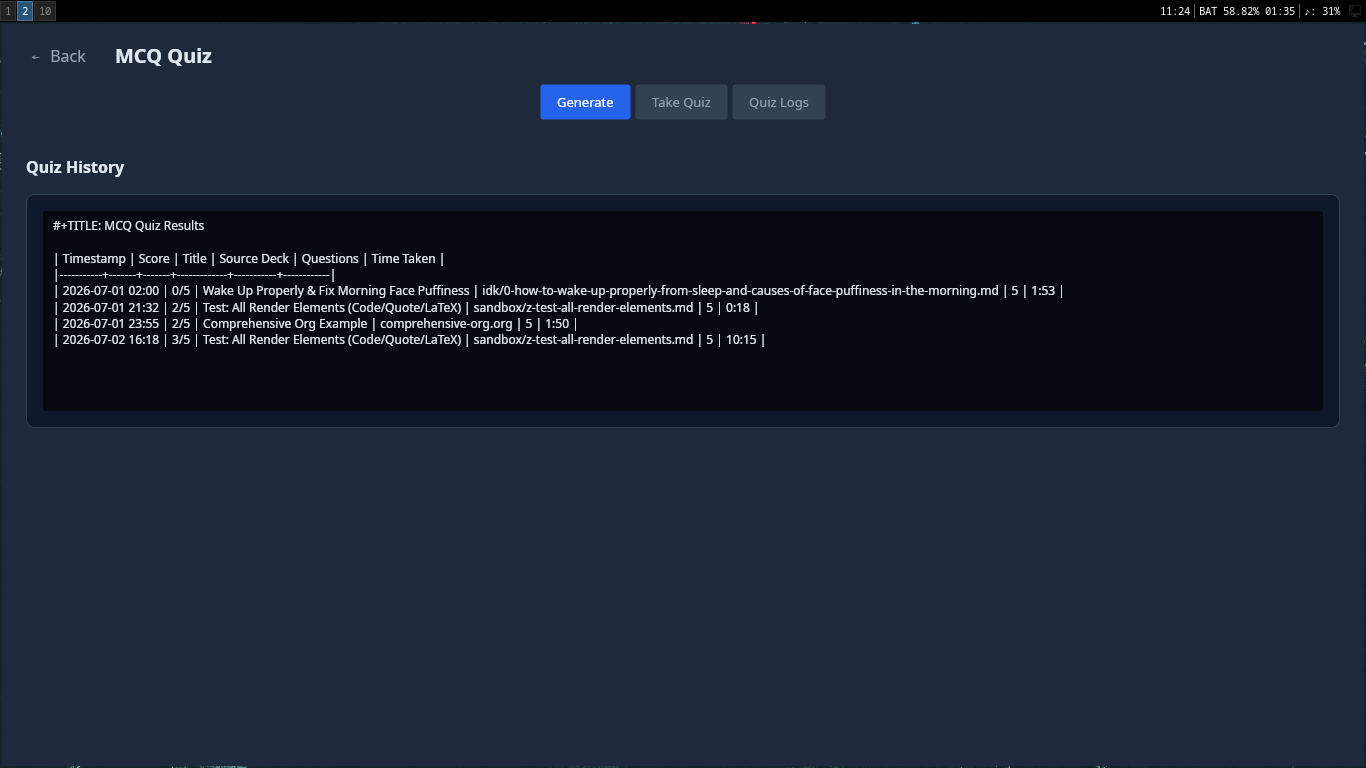
\includegraphics[width=550]{./screenshots/mcq-quiz-logs-tab.png}
\end{center}

\textbf{Figure 22: MCQ quiz logs tab — review past quiz results and performance.}
\subsubsection{Theme System}
\label{sec:orgb16d497}
\begin{center}
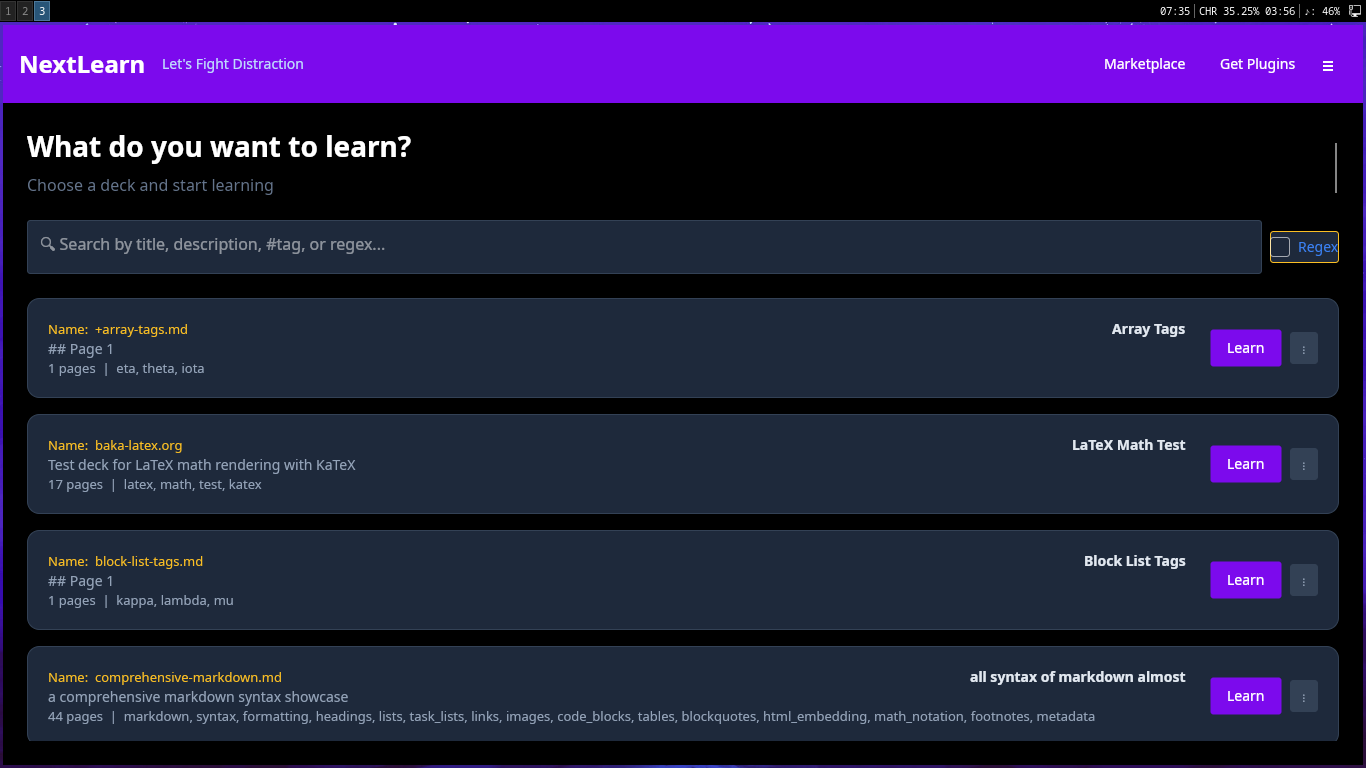
\includegraphics[width=550]{./screenshots/default-dark-theme.png}
\end{center}

\textbf{Figure 23: The updated default dark theme.}

\begin{center}
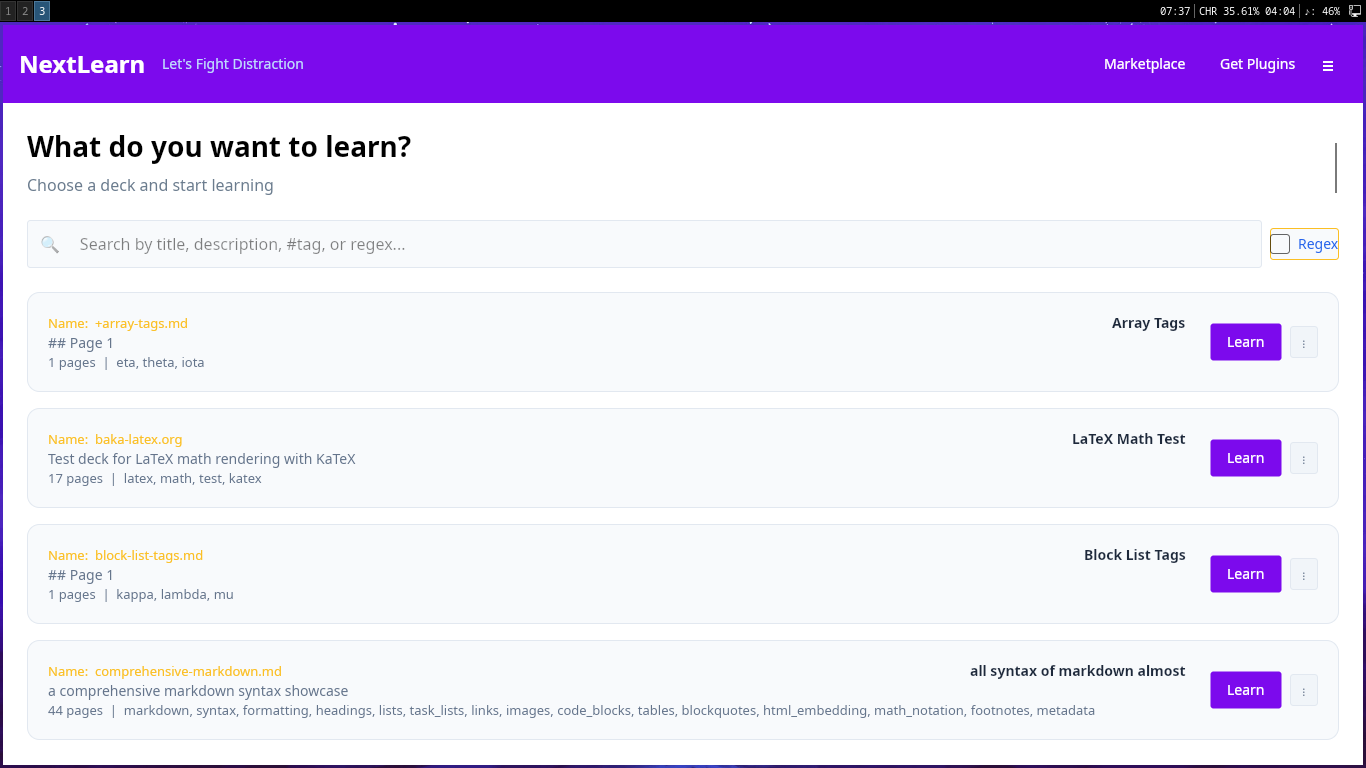
\includegraphics[width=550]{./screenshots/default-light-theme.png}
\end{center}

\textbf{Figure 24: Default light theme.}

\begin{center}
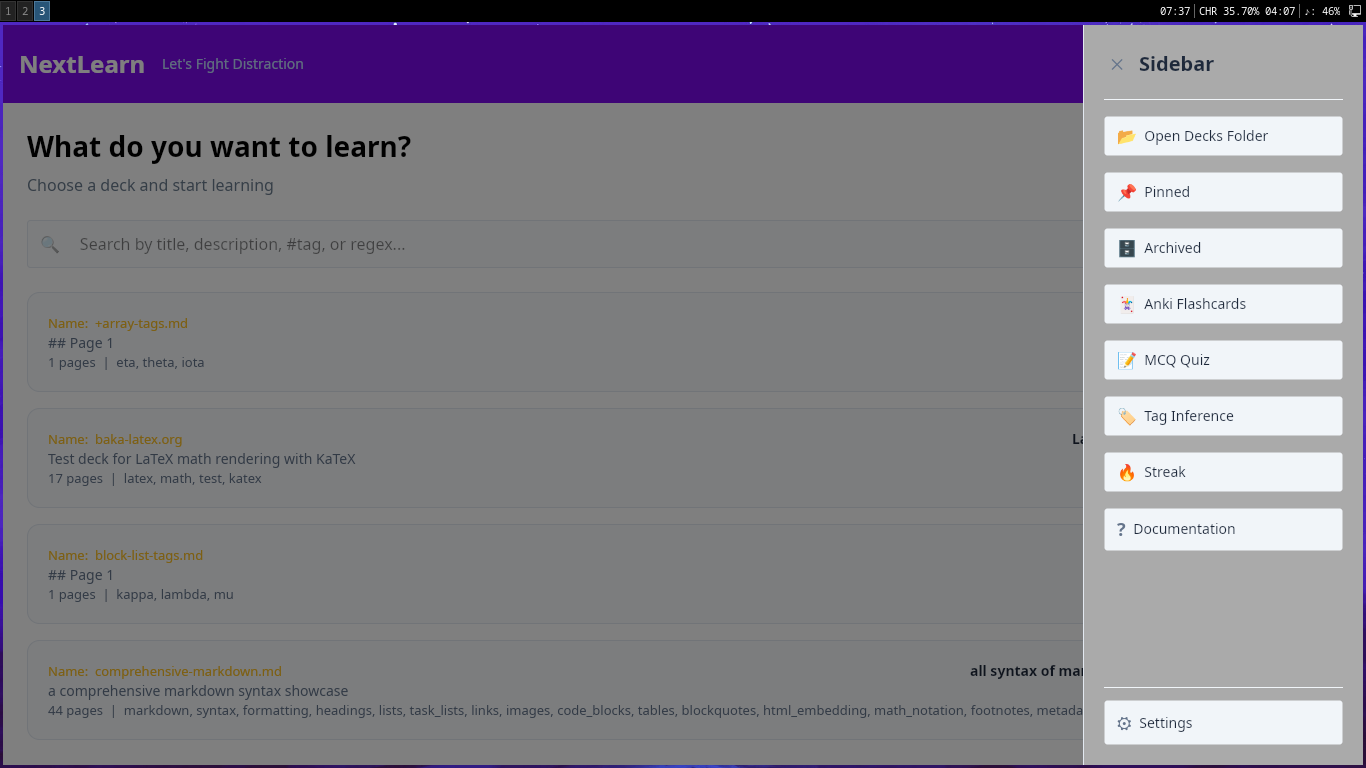
\includegraphics[width=550]{./screenshots/default-light-theme-sidebar.png}
\end{center}

\textbf{Figure 25: Sidebar in light theme.}

\begin{center}
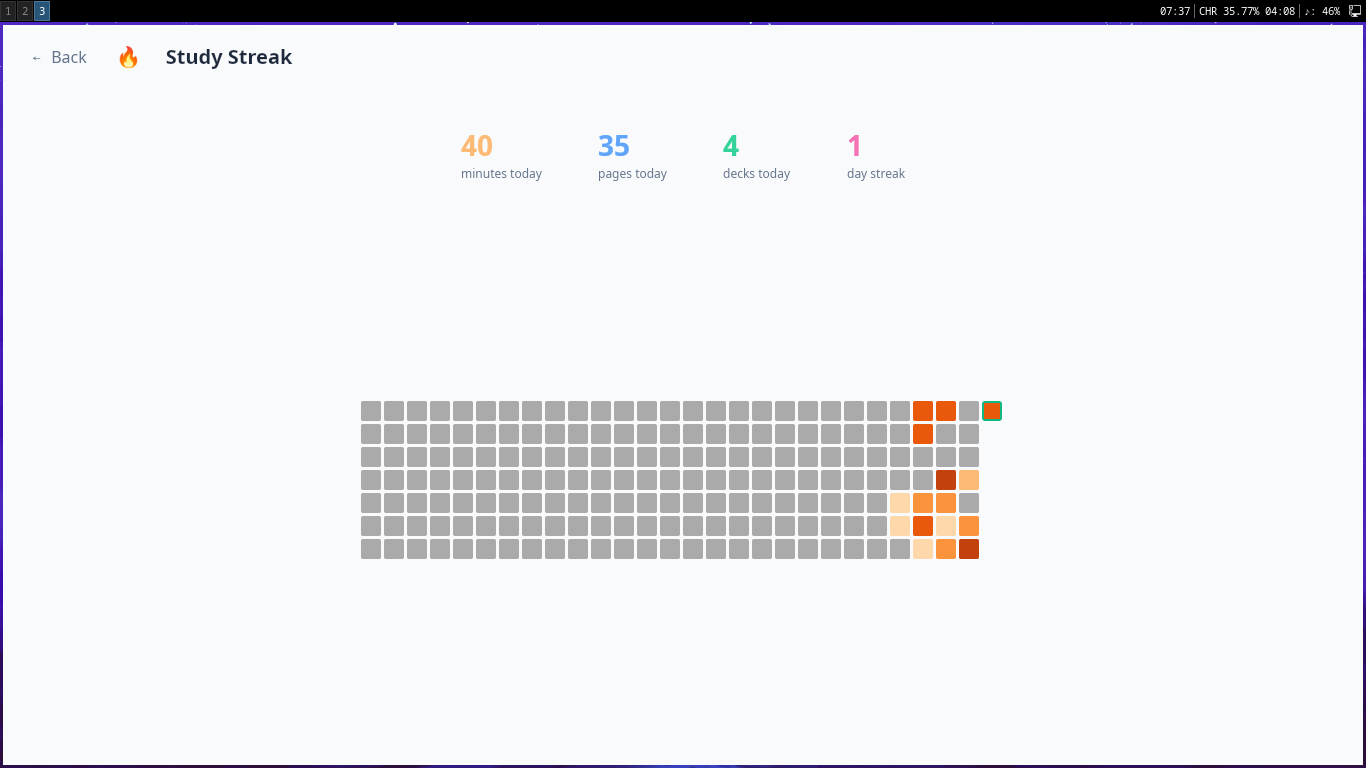
\includegraphics[width=550]{./screenshots/default-light-theme-heatmap.png}
\end{center}

\textbf{Figure 26: Heatmap in light theme.}
\subsubsection{Focus Timer}
\label{sec:orga01b3bc}
\begin{center}
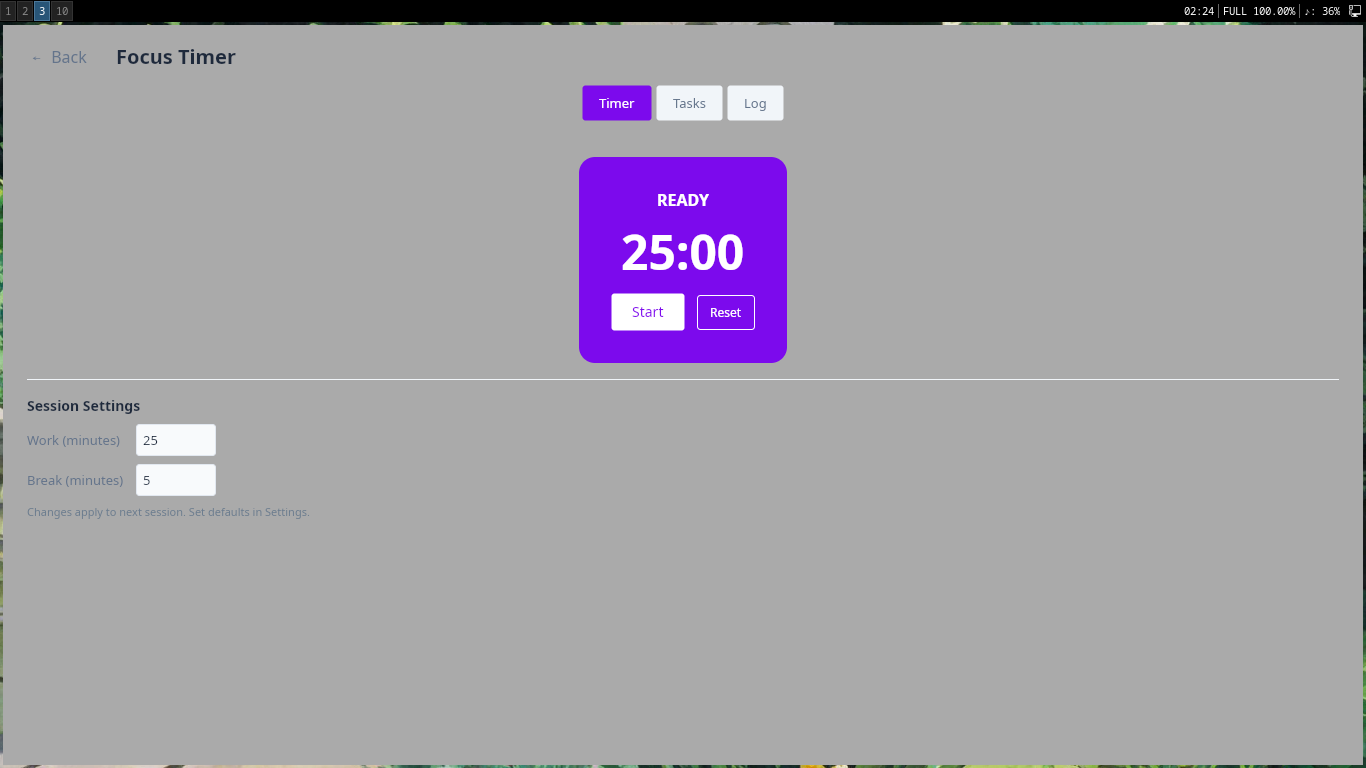
\includegraphics[width=550]{./screenshots/focus-timer-panel.png}
\end{center}

\textbf{Figure 27: Focus timer panel — Pomodoro timer, tasks CRUD, and session history.}

\newpage
\subsection{Theme System}
\label{sec:orge1f35f0}
NextLearn features a live-switchable dark/light theme system with 45+
named resource keys defined in \texttt{ThemeHelper.cs}.
\subsubsection{Architecture}
\label{sec:org850efff}
\begin{enumerate}
\item All colors centralized as named resources (\texttt{PageBgBrush},
\texttt{TextPrimaryBrush}, etc.) in \texttt{App.axaml → Application.Resources}
\item All 13 \texttt{.axaml} files refactored from inline hex to
\texttt{\{StaticResource ResourceKey}\ldots{}\}=
\item \texttt{ThemeHelper.cs} contains two dictionaries

(\texttt{DarkColors} and \texttt{LightColors}) with \texttt{ApplyTheme(string? theme)} method
\item Theme setting persisted in \texttt{settings.yaml}
\end{enumerate}
\subsubsection{Color Palettes}
\label{sec:org2c05050}
\begin{center}
\begin{tabular}{lll}
Resource Key & Dark Value & Light Value\\
\hline
\texttt{PageBgBrush} & \#0F172A & \#F8FAFC\\
\texttt{PanelBgBrush} & \#1E293B & \#FFFFFF\\
\texttt{SurfaceBgBrush} & \#334155 & \#F1F5F9\\
\texttt{TextPrimaryBrush} & \#E2E8F0 & \#1E293B\\
\texttt{TextSecondaryBrush} & \#94A3B8 & \#64748B\\
\texttt{TextMutedBrush} & \#64748B & \#94A3B8\\
\texttt{BorderDefaultBrush} & \#334155 & \#E2E8F0\\
\texttt{ButtonSecondaryBgBrush} & \#334155 & \#E2E8F0\\
\texttt{AccentBrush} & \#7C0AED & \#7C0AED\\
\end{tabular}
\end{center}

Complementary colors (green for today, warning amber, etc.) maintain
readability across both themes.

\newpage
\section{Proposed Workflow}
\label{sec:org4f27448}
This section describes the intended end-to-end workflow for a typical
user session with NextLearn.
\subsection{Typical Evening Study Session}
\label{sec:orgb0c86a8}
\begin{enumerate}
\item \textbf{\textbf{Launch}}: User starts NextLearn. The app creates a guest user
(first run), scans the \texttt{\textasciitilde{}/nextlearn/decks/} directory recursively,
syncs file metadata with the SQLite database, and displays the deck
list on the Home screen.

\item \textbf{\textbf{Search and Select}}: User types \texttt{\#programming} in the search bar
to filter decks tagged with "programming". The deck list narrows
in real-time.

\item \textbf{\textbf{Start Study}}: User presses \texttt{Enter} on the selected deck. The
app loads the deck file, parses it into pages, builds HTML with
KaTeX/highlight.js enrichment, and displays the first page in the
WebView.

\item \textbf{\textbf{Navigate}}: User reads through pages using \texttt{N} (next) and \texttt{P}
(previous). The section breadcrumb shows current position:
\texttt{"Data Structures → Binary Trees "}. Progress is saved to the
database after each page navigation.

\item \textbf{\textbf{Deep Work}}: User activates the Focus Timer (sidebar → Timer,
or command palette). Starts a 25-minute Pomodoro session. The
study box content is still visible. Timer counts down with a
sound notification at session end.

\item \textbf{\textbf{Generate Flashcards}}: After studying, user opens the Flashcard
panel, clicks \texttt{Cloze} on the current deck. Gemini generates
fill-in-the-blank cards. User reviews and accepts → saved as
\texttt{binary-trees.cloze.txt} for Anki import.

\item \textbf{\textbf{Self-Assessment}}: User opens the MCQ Quiz panel, generates 10
questions from the deck via Gemini. Takes the interactive quiz
in the dedicated WebView — 2×2 option grid, timer running.
Review the score summary at the end.

\item \textbf{\textbf{Review Progress}}: User opens the Heatmap overlay (Ctrl+H).
The snake-layout heatmap shows the past 12 months of study
activity. Today's cell is green. Current streak is displayed.

\item \textbf{\textbf{Exit}}: User closes the app. All progress is persisted. The
focus timer session was logged, the heatmap was updated, and
the quiz results were saved as \texttt{.mcq.result} files.
\end{enumerate}

\newpage
\subsection{Alternative Workflows}
\label{sec:org5dbca62}
\begin{itemize}
\item \textbf{\textbf{New Deck Creation}}: User creates a \texttt{.md} file outside the app
(Vim, Emacs, VS Code), saves it to \texttt{\textasciitilde{}/nextlearn/decks/}. The app
auto-refreshes (FileSystemWatcher, 300ms debounce) and the new
deck appears in the list.

\item \textbf{\textbf{Deck Editing}}: User modifies a deck file externally. Next
time the deck is opened, the app reads the latest file content.
Progress is linked by SHA256 identity — renaming the file does
not lose progress.

\item \textbf{\textbf{Tag Maintenance}}: User opens the Tag Inference panel, selects
a deck that has no tags, clicks "Infer Tags". Gemini suggests
5 tags. User reviews, removes one, applies the remaining 4 —
the tags are written to the YAML frontmatter preserving the
original format.

\item \textbf{\textbf{Cross-Deck Navigation}}: While studying a deck, user clicks a
wiki-link \texttt{[[related topic]]}. The app checks for the target
deck (.md → .org fallback), shows a prompt, and navigates to
the linked deck's first page.
\end{itemize}
\section{Limitations \& Risk Analysis}
\label{sec:orgd238311}
\subsection{Linux WebView Constraint}
\label{sec:orgfa31808}
\begin{itemize}
\item \textbf{\textbf{Issue}}: NativeWebView on Linux depends on \texttt{libwpewebkit-2.0} and
related WPE WebKit libraries. These are available on major
distributions but may not be pre-installed.
\item \textbf{\textbf{Windows}}: Not currently supported — requires WebView2 runtime
while the app uses the system WebView API available on Linux.
\item \textbf{\textbf{Mitigation}}: Wayland detection with X11 fallback in Program.cs.
clear error messages for missing dependencies.
\item \textbf{\textbf{Risk}}: Low (Linux is the primary target). Windows support would
require a separate WebView backend (e.g., WebView2).
\end{itemize}

\newpage
\subsection{Google Gemini API Dependency}
\label{sec:orgf0a0247}
\begin{itemize}
\item \textbf{\textbf{Issue}}: AI features (tag inference, flashcards, MCQ generation)
require a Google Gemini API key and internet connectivity.
\item \textbf{\textbf{Rate Limits}}: Free tier has quota limits. The app implements
exponential retry (1s, 5s, 10s, 20s, 40s, 80s) and model fallback
chain, but extended outages break AI features.
\item \textbf{\textbf{Mitigation}}: All AI features are optional. The core study
functionality works fully offline. API responses are saved as local
files — the user is never locked into any AI provider.
\item \textbf{\textbf{Risk}}: Low (AI is additive, not required).
\end{itemize}
\subsection{Single-User Offline Model}
\label{sec:org74733cc}
\begin{itemize}
\item \textbf{\textbf{Issue}}: No multi-user support, no cloud sync, no authentication.
\item \textbf{\textbf{Mitigation}}: By design — the application targets individual
learners who value privacy and data ownership over collaboration.
File-based format makes manual sync trivial (git, rsync, Dropbox).
\item \textbf{\textbf{Risk}}: Acceptable for the project scope.
\end{itemize}

\newpage
\subsection{No Automated UI Tests}
\label{sec:org4f54897}
\begin{itemize}
\item \textbf{\textbf{Issue}}: The test suite covers service and parser logic but has
no UI automation tests (Avalonia UI testing framework not integrated).
\item \textbf{\textbf{Mitigation}}: ViewModels contain minimal logic — most complexity
is in Services layer which is well-tested.
\item \textbf{\textbf{Risk}}: Low-medium. UI bugs are caught manually during development.
\end{itemize}
\subsection{Performance on Very Large Decks}
\label{sec:org2f9ed5d}
\begin{itemize}
\item \textbf{\textbf{Issue}}: Single HTML string built for entire deck content could
be slow for decks with 1000+ pages.
\item \textbf{\textbf{Mitigation}}: Current usage targets decks of 10--100 pages.
Token estimation in AI services warns at >700K tokens.
\item \textbf{\textbf{Risk}}: Low — file-based architecture makes it easy to split
large decks into multiple files.
\end{itemize}

\newpage
\section{Conclusion \& Future Work}
\label{sec:org1fbbf77}
\subsection{Conclusion}
\label{sec:org4350a20}
\begin{center}
NextLearn demonstrates that a single developer can build a
professional-grade, distraction-free study environment using free and
open-source tools. The project's file-first architecture ensures that
users own their data in plain text. The keyboard-centric design,
inspired by Vim and Emacs, provides a mouse-free experience unmatched
by mainstream study applications. The optional AI integration via
Google Gemini adds modern convenience without compromising local
control.


\end{center}
\begin{center}
The project is currently in active development with all core features
implemented: deck management, paginated study, image rendering, LaTeX
math, code syntax highlighting, AI tag inference, flashcard
generation, interactive MCQ quizzes, a focus timer, and streak
tracking. The application builds and runs on Linux (primary) and
macOS, with GitHub Actions CI ensuring cross-platform compatibility.


\end{center}
\begin{center}
At approximately 20,000+ lines of code across 41 service files, 13
ViewModels, 14 user controls, and 6 database tables, NextLearn is a
substantial software engineering project that applies modern .NET
practices (MVVM, EF Core, dependency injection preparation, structured
logging, YAML configuration) to a focused domain problem.

\end{center}
\newpage
\subsection{Future Potential Work \& Features}
\label{sec:orgf7e2db0}
\begin{itemize}
\item Decide business model:
\begin{itemize}
\item Free / Paid?
\item /perma, /verified, /notverified, /perma-verified
\item How long would hosting last for each tier?
\end{itemize}
\item llms.txt for the website
\item Plugin system — Scriptable extensions (JavaScript/Python/csharp\ldots{}etc plugins).
\begin{itemize}
\item Hamburger menu should list installed plugins
\item Plugin: background lofi music player
\item Plugin: theme switcher (user-editable CSS override)
\end{itemize}
\item Built-in: nextsnipe, snipes notes from within the file
\item Keybinding: \texttt{i} in all profiles → opens image overlay on first image in study box
\item Markdig (markdown parser replacement?)
\item OCR in image overlay
\item Image overlay annotations with live updates:
\begin{itemize}
\item Option A: button that refreshes/re-reads the image
\item Option B: live image update (filesystem watcher)
\end{itemize}
\item Evaluate YAML → TOML format migration
\item Copy button missing on \LaTeX{} blocks in Anki Flashcard panel (Basic / Cloze prompts)
\end{itemize}
\newpage
\begin{itemize}
\item Marketplace — browse and download community decks (placeholder exists)
\item Theme presets / custom themes — user-defined color schemes
\item Spaced repetition — basic 24h review → full SRS (SM-2 or FSRS)
\item Mobile companion — PWA or MAUI
\item Multi-user profiles — switchable within the app
\item Anki direct sync — two-way sync via AnkiConnect
\item Export formats — PDF, EPUB, HTML single-page
\item Plugin system — scriptable extensions (JS/Python)
\item Real-time collaboration — shared study sessions
\item Audio support — text-to-speech
\item Gamification — achievements, levels, leaderboards (optional)
\item AI model flexibility — local LLMs (Ollama, llama.cpp) + alternative providers
and alternative providers (Anthropic, OpenAI).
\item Windows support — WebView2 backend for cross-platform
\item Mobile app — native iOS/Android via Avalonia MAUI
\end{itemize}


\newpage
\section{References \& Inspiration}
\label{sec:orgc4067a7}
\subsection{Technology References}
\label{sec:orgc2afbd7}
\begin{itemize}
\item Avalonia UI: \url{https://avaloniaui.net/} — Cross-platform desktop UI
framework for .NET
\item CommunityToolkit.Mvvm: \url{https://learn.microsoft.com/en-us/dotnet/communitytoolkit/mvvm/}
— Source-generated MVVM pattern
\item Entity Framework Core: \url{https://learn.microsoft.com/en-us/ef/core/}
— ORM for .NET
\item Serilog: \url{https://serilog.net/} — Structured logging
\item YamlDotNet: \url{https://github.com/aaubry/YamlDotNet} — YAML serialization
\item highlight.js: \url{https://highlightjs.org/} — Syntax highlighting (52 languages)
\item KaTeX: \url{https://katex.org/} — Fast \LaTeX{} math rendering
\item Google Gemini API: \url{https://ai.google.dev/} — AI model API
\item NativeWebView: \url{https://github.com/arthurrump/NativeWebView} —
Avalonia WebView control
\item xUnit: \url{https://xunit.net/} — Unit testing framework
\item FluentAssertions: \url{https://fluentassertions.com/} — Readable test assertions
\item NSubstitute: \url{https://nsubstitute.github.io/} — Mocking framework
\end{itemize}

\newpage
\subsection{Design Inspiration}
\label{sec:orgac57210}
\begin{itemize}
\item \textbf{\textbf{Anki}} (\url{https://apps.ankiweb.net/}) — Spaced repetition flashcard
system
\item \textbf{\textbf{Obsidian}} (\url{https://obsidian.md/}) — Markdown knowledge base with
wiki-links and vault concept and bidirectional links
\item \textbf{\textbf{SuperMemo}} (\url{https://supermemo.guru/}) — Early SRS pioneer
\item \textbf{\textbf{Vim}} (\url{https://www.vim.org/}) — Modal text editing with keyboard
shortcuts
\item \textbf{\textbf{Neovim}} (\url{https://www.neovim.io/}) — The community child of vim
\item \textbf{\textbf{GNU Emacs}} (\url{https://www.gnu.org/software/emacs/}) — Extensible
editor with chord-based keybindings
\item \textbf{\textbf{Visual Studio Code}} (\url{https://code.visualstudio.com/}) — Modern
editor keybinding conventions
\item \textbf{\textbf{goyo.vim}} (\url{https://github.com/junegunn/goyo.vim}) Distraction-free writing in Vim
\end{itemize}

\newpage
\section{License \& Source Code}
\label{sec:org76e2fcc}
\subsection{License}
\label{sec:orgeadabf9}
This project is currently distributed without an explicit license file.
All rights reserved by the author. Users may view and build the source
code for personal use. A permissive open-source license (MIT) is planned
for future release.
\subsection{Source Code}
\label{sec:org237026b}
Repository: \url{https://github.com/megamind1230/nextlearn}

Branch: main (default branch)

The repository contains:

\begin{itemize}
\item \texttt{NextLearn.Desktop/} — Avalonia UI desktop application
\item \texttt{tests/NextLearn.Desktop.Tests/} — xUnit unit tests
\item \texttt{screenshots/} — Application screenshots gallery
\item \texttt{.github/workflows/ci.yml} — GitHub Actions CI configuration
\item Documentation files: \texttt{README.org}, \texttt{DOCUMENTATION.org},
\texttt{changelog.org}, \texttt{plan-todos.org}, \texttt{bugs.org}, \texttt{screenshots.org}
\end{itemize}

Build instructions:
\begin{verbatim}
git clone https://github.com/megamind1230/nextlearn
cd testing-nextlearn
dotnet build NextLearn.Desktop/NextLearn.Desktop.csproj -c Release
dotnet run --project NextLearn.Desktop
\end{verbatim}

To produce a portable single-file binary:
\begin{verbatim}
dotnet publish NextLearn.Desktop/NextLearn.Desktop.csproj \
  -c Release \
  -r linux-x64 \
  --self-contained true \
  -p:PublishSingleFile=true \
  -o publish
\end{verbatim}
\end{document}
